\documentclass[10pt,twocolumn,letterpaper]{article}
\usepackage[review]{cvpr}
\usepackage{tabularx}
\usepackage{array}
\definecolor{cvprblue}{rgb}{0.21,0.49,0.74}
\usepackage[breaklinks,colorlinks,allcolors=cvprblue]{hyperref}
\def\confName{CVPR}
\def\confYear{2027}
\def\cvprPaperID{TBD}
\title{Contact-Informed Visuomotor Interface:\\
Learning Force--Vision Fusion in Image Space for Contact-Rich Manipulation}
\author{Anonymous CVPR submission}
\graphicspath{{assets/}}
\newcommand{\civi}{\textsc{Civi}\xspace}
\newcommand{\dpkey}{\textsc{DP}\xspace}
\newcommand{\pizero}{$\pi_0$\xspace}
\renewcommand{\thesection}{S\arabic{section}}
\renewcommand{\thesubsection}{S\arabic{section}.\arabic{subsection}}
\renewcommand{\thetable}{S\arabic{table}}
\renewcommand{\thefigure}{S\arabic{figure}}

\begin{document}
\maketitlesupplementary

This supplement expands the method, evaluation protocol, and diagnostics for
the paper. Section~\ref{sec:method} gives the complete causal interface and
training objectives. Section~\ref{sec:protocol} specifies the real-robot
protocol and reports the per-task results and costs. Section~\ref{sec:alignment}
provides the representation-alignment and component ablations. Section~\ref{sec:causal}
reports causal phase and torque interventions. Section~\ref{sec:limits} records
negative controls and evidence limits. Sections~\ref{sec:visual_evidence}--
\ref{sec:paired_extra} add repository robot, renderer, phase, torque-estimation,
and paired-response visualizations. Section~\ref{sec:fusion_probes} compares
three teacher fusion operators on recorded robot data and relates their
attention maps to changes in context and action. Section~\ref{sec:sim_real}
reports simulation and robot training results, including a LIBERO rollout evaluation.

\section{Method Details}
\label{sec:method}

\subsection{Causal torque history and phase switch}
\label{sec:method_phase}
Let $q_t$, $\dot q_t$, and $\tau_{m,t}$ be joint position, velocity, and
measured motor torque. NEXT estimates the free-motion torque from the most
recent proprioceptive history, and the external torque is the residual
\begin{equation}
 \widehat{\tau}^{\,\mathrm{free}}_t=f_{\mathrm{NEXT}}([q,\dot q,\Delta q]_{t-L+1:t}),\qquad
 \widehat{\tau}^{\,\mathrm{ext}}_t=\tau_{m,t}-\widehat{\tau}^{\,\mathrm{free}}_t.
 \label{eq:next}
\end{equation}
The signed vector is retained by the model. Its $\ell_1$ magnitude is used
only to construct the phase reference. Thresholding with temporal persistence
gives $s_t\in\{\mathrm{free},\mathrm{pre},\mathrm{contact}\}$. Non-contact
frames in the 0.5-second interval before a confirmed onset are labelled
pre-contact. The binary training switch is
\begin{equation}
 b_t=\mathbb{1}[s_t\in\{\mathrm{pre},\mathrm{contact}\}].
 \label{eq:phase}
\end{equation}
The deployment switch is predicted from causal observations $O_{\leq t}$,
$\widehat b_t=\mathbb{1}[C_\eta(O_{\leq t})\in\{\mathrm{pre},\mathrm{contact}\}]$.
The deployed interface uses measurements through time $t$. The phase-gate
diagnostic uses a 50-frame, 25-Hz torque history
(approximately 2 seconds), a 12.5-Nm $\ell_1$ threshold, and five-frame
persistence. The signed history, rather than its magnitude, is passed to the
teacher and renderer.

\subsection{Action-supervised teacher}
\label{sec:method_teacher}
The frozen DINOv3 image encoder produces patch tokens $P_t$. An LSTM encodes
the signed history $T_t=[\widehat\tau^{\,\mathrm{ext}}_{t-K+1},\ldots,
\widehat\tau^{\,\mathrm{ext}}_t]$ as $H_t^\tau$. Two residual cross-attention
blocks use visual tokens as queries and torque features as keys and values.
The fused context is
\begin{equation}
 Z_t^T=\operatorname{LN}\!\left(P_t+b_t[\mathcal F(P_t,H_t^\tau)-P_t]\right).
 \label{eq:teacher}
\end{equation}
All views and observation steps are concatenated before conditioning the
diffusion transformer. We use the standard noise-prediction objective
\begin{equation}
 \mathcal L_{\mathrm{teacher}}=\mathbb E\left[\|D_\psi(A_t^{(n)},n,Z_t^T)-\epsilon\|_2^2\right].
 \label{eq:teacher_loss}
\end{equation}

During the teacher curriculum, selected pre-contact and contact visual patch
tokens are replaced by a shared mask token. The probability is one during the
first quarter of training, decreases linearly over the middle half, and is
zero during the final quarter. Free-motion tokens remain visible. This
curriculum encourages interaction-phase torque use while preserving ordinary
visual control in free motion. The teacher is frozen before renderer targets
are constructed.

\begin{figure*}[t]
  \centering
  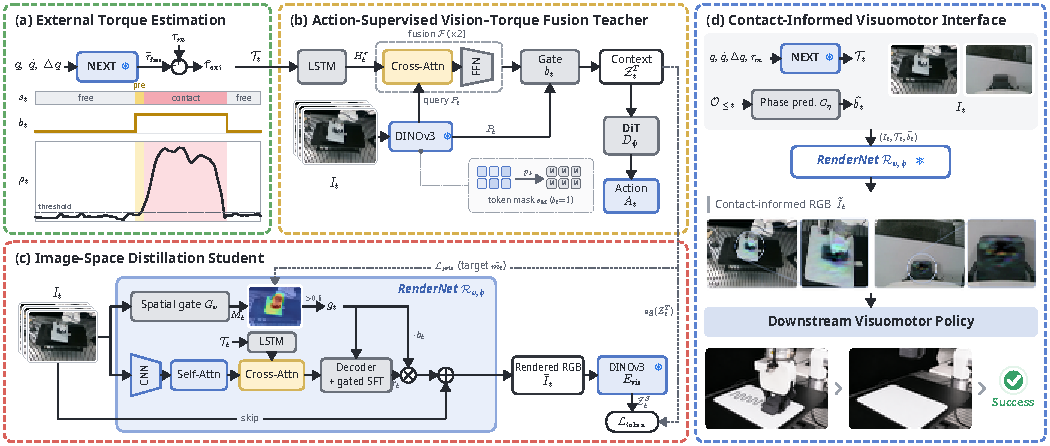
\includegraphics[width=0.96\textwidth]{method_overview_v2.pdf}
  \caption{CIVI overview, including proprioceptive external-torque estimation,
  action-supervised vision--torque fusion, image-space distillation, and the
  causal deployment path.}
  \label{fig:arch}
\end{figure*}

\subsection{Image-space distillation}
\label{sec:method_student}
The student has a spatial gate $G_\omega$ and an RGB residual branch
$U_\phi$. For a clear image $I_t$, the teacher's visual-only context is
$Z_t^0=\operatorname{LN}(P_t)$ and its fused context is $Z_t^T$. The patchwise
fusion effect defines
\begin{equation}
 d_{t,j}=\|Z^T_{t,j}-Z^0_{t,j}\|_2,\qquad
 \bar m_{t,j}=\frac{d_{t,j}-\min_jd_{t,j}}
 {\max_jd_{t,j}-\min_jd_{t,j}+\varepsilon}.
 \label{eq:mask_target}
\end{equation}
The gate is trained against $\bar m_t$ with a Smooth-$\ell_1$ term and total
variation. After gate pretraining, its weights are fixed. The thresholded gate
is $g_t=M_t\odot\mathbb 1[M_t>0.5]$. At two decoder resolutions, feature
transforms are applied as
\begin{equation}
 f'_\ell=f_\ell+g_{t,\ell}\odot(\gamma_\ell\odot f_\ell+\beta_\ell).
 \label{eq:sft}
\end{equation}
The RGB branch predicts a residual $r_t$ and produces
\begin{equation}
 \widetilde I_t=\operatorname{clip}_{[0,1]}\left(I_t+b_tg_t\odot\tanh(r_t)\right).
 \label{eq:render}
\end{equation}
Consequently, free motion recovers the input image exactly. The rendered image
is encoded by the frozen visual pathway $E_{\mathrm{vis}}$, and only the RGB
branch is optimized with
\begin{equation}
 \mathcal L_{\mathrm{token}}=\frac{1}{Nd}\|E_{\mathrm{vis}}(\widetilde I_t)-\operatorname{sg}(Z_t^T)\|_F^2.
 \label{eq:token_loss}
\end{equation}
The gate target and teacher context are detached. After distillation, the
renderer is frozen for downstream policy training and deployment.

\begin{figure}[t]
  \centering
  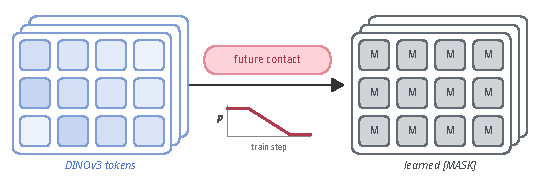
\includegraphics[width=\columnwidth]{image_token_mask.pdf}
  \caption{Teacher-training curriculum. A learned mask token replaces selected
  visual patches on contact-related observations during training. The separate
  spatial target for the renderer is defined in Eq.~\ref{eq:mask_target}.}
  \label{fig:mask}
\end{figure}

\section{Experimental Protocol and Main Results}
\label{sec:protocol}

\subsection{Tasks, data, and success rules}
\label{sec:tasks}
We evaluate on three contact-rich tasks with an xArm robot. Each task has 45
demonstrations. Wipe Board and Peel Cucumber cover three working heights.
The success rule is task completion, namely all target markings removed,
more than 8 cm of cucumber skin peeled, or the circuit breaker fully toggled.
The wrist and external cameras are used together with the estimated external
torque. Each method is evaluated on 20 trials under the same initial-condition
distribution.

\begin{table}[t]
\centering
\caption{Closed-loop success counts. Each entry is successes out of 20 trials.}
\label{tab:success}
\setlength{\tabcolsep}{3.6pt}
\resizebox{\columnwidth}{!}{%
\begin{tabular}{@{}lrrrrr@{}}
\toprule
Task & \pizero RGB & \pizero CIVI & \dpkey RGB & \dpkey CIVI & TA-VLA \\
\midrule
Wipe Board & 11 & 14 & 4 & 10 & 12 \\
Peel Cucumber & 12 & 16 & 6 & 9 & 15 \\
Open Switch & 8 & 13 & 4 & 6 & 11 \\
\midrule
Pooled / 60 & 31 & 43 & 14 & 25 & 38 \\
Success (\%) & 51.7 & 71.7 & 23.3 & 41.7 & 63.3 \\
\bottomrule
\end{tabular}
}
\end{table}

The same frozen task-specific renderer is shared by the two downstream
policies. The RGB and CIVI policies retain their original visual encoders,
action objectives, action horizons, and low-level controllers. DP uses DDPM
sampling for the success table. TA-VLA is an in-policy torque-fusion baseline.
The pooled 95\% Wilson intervals are 39.3--63.8\% for RGB \pizero,
59.2--81.5\% for CIVI \pizero, 14.4--35.4\% for RGB DP, 30.1--54.3\% for
CIVI DP, and 50.7--74.4\% for TA-VLA. These intervals describe the 60 pooled
trials and do not account for shared initial-condition blocks.

\subsection{Latency and training cost}
\label{sec:cost}
Latency is the median policy-call time on one RTX 5090 with batch size one and
two cameras, excluding image capture and transfer. The renderer executes once
per policy call and is independent of the number of diffusion denoising steps.

\begin{table}[t]
\centering
\caption{Deployment latency. The number in parentheses is the absolute CIVI
overhead in milliseconds.}
\label{tab:latency}
\setlength{\tabcolsep}{3.8pt}
\resizebox{\columnwidth}{!}{%
\begin{tabular}{@{}lrrr@{}}
\toprule
Policy & Sampler & RGB (ms) & RGB+CIVI (ms) \\
\midrule
DP & DDPM-50 & 132.6 & 143.6 (+11.0) \\
DP & DDIM-8 & 26.0 & 38.4 (+12.4) \\
\pizero & 10 steps & 436 & 458 (+22) \\
\bottomrule
\end{tabular}
}
\end{table}

On the same RTX 5090, teacher training and renderer distillation take about
6 and 2 GPU hours per task. A downstream DP policy takes about 6 GPU hours and
\pizero fine-tuning about 8 GPU hours, matching their RGB counterparts. The
renderer is trained once per task and then reused by both policy families.

\begin{figure}[t]
  \centering
  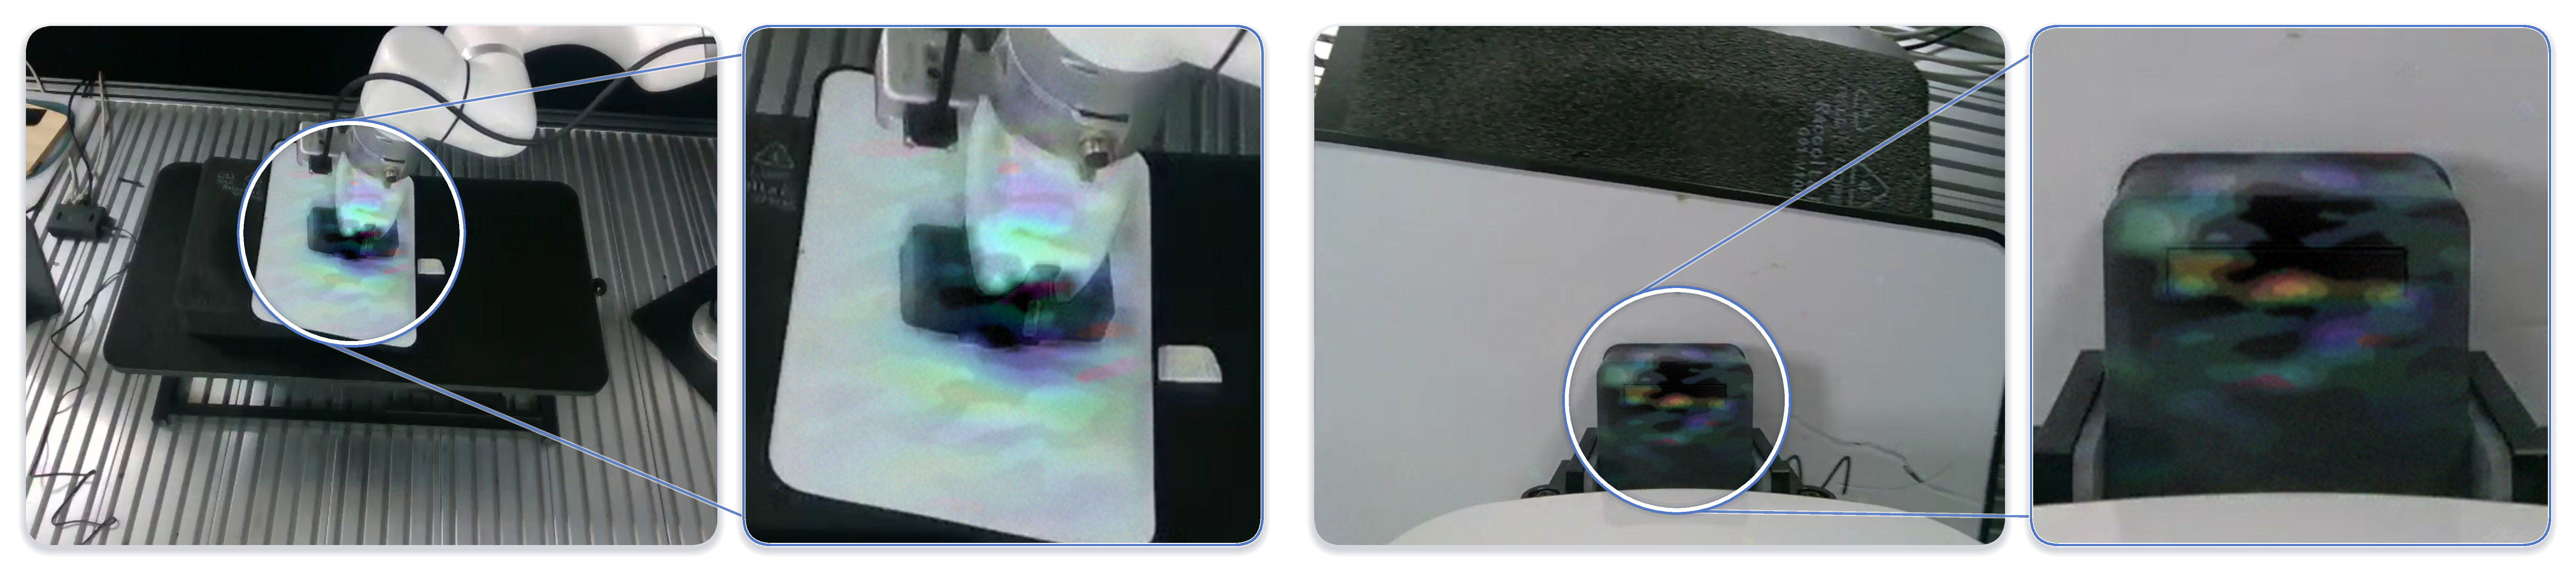
\includegraphics[width=\columnwidth]{render_zoom_row.pdf}
  \caption{Illustrative image-space render and zoom visualization included
  with the method assets. This is a schematic rendering illustration, not a
  frame from the real-robot diagnostics in Sec.~\ref{sec:visual_evidence}.}
  \label{fig:render}
\end{figure}

\section{Representation Alignment and Ablations}
\label{sec:alignment}

\subsection{Image-space alignment}
The LIBERO drawer-and-bowl student reproduces the 53.8\% all-token and
53.9\% fusion-active reductions in the main paper. Its teacher receives eight
future force/torque samples. The reference is the identity RGB path at the
first validation epoch. Table~\ref{tab:alignment_domains} gives the absolute
errors and the corresponding real-board runs. The real-robot component
ablation in Table~\ref{tab:ablation} uses its own task-specific windows.

\begin{figure*}[t]
  \centering
  \begin{subfigure}[t]{0.49\textwidth}
    \centering
    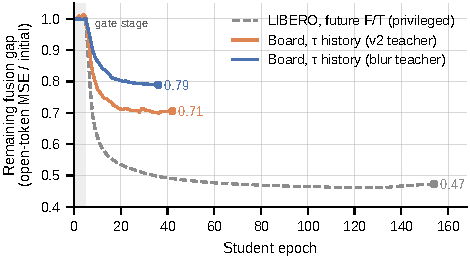
\includegraphics[width=\linewidth]{distillation_gap.pdf}
    \caption{Open-token validation MSE relative to each run's first epoch.}
  \end{subfigure}
  \hfill
  \begin{subfigure}[t]{0.49\textwidth}
    \centering
    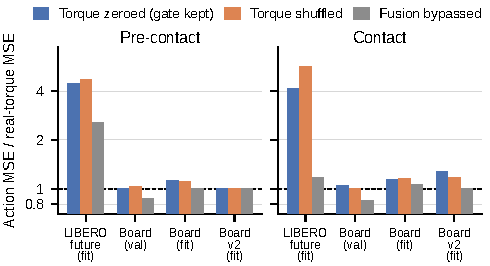
\includegraphics[width=\linewidth]{torque_reliance.pdf}
    \caption{Teacher response to torque interventions.}
  \end{subfigure}
  \caption{Additional diagnostics generated from the repository experiment
  records. They are offline representation measurements and do not replace
  the closed-loop success evaluation.}
  \label{fig:diagnostics}
\end{figure*}

\subsection{Spatial component ablation}
\label{sec:ablation}
The two spatial components are ablated with the same trained renderer and
identical input windows. Decoder SFT is bypassed at inference while retaining
the gate. For the mask ablation, the spatial gate is replaced by ones in both
SFT and the final residual while contact gating is retained. We report relative
error reduction against the corresponding ablation, so higher is better.

\begin{table*}[t]
\centering
\caption{Spatial component ablation. Values are relative error reductions
(\%) on rendering-active validation windows. Action MSE is in normalized action
space and position is end-effector RMSE.}
\label{tab:ablation}
\setlength{\tabcolsep}{4.0pt}
\begin{tabular}{@{}llrrrrrrrrr@{}}
\toprule
 & & \multicolumn{3}{c}{Wipe Board} & \multicolumn{3}{c}{Peel Cucumber} & \multicolumn{3}{c}{Open Switch} \\
Component & Metric & Context & Action & Pos. & Context & Action & Pos. & Context & Action & Pos. \\
\midrule
Decoder SFT & error reduction & 42.2 & 12.6 & 11.7 & 46.4 & 15.9 & 10.2 & 38.9 & 13.3 & 10.3 \\
Spatial mask $M$ & error reduction & 54.7 & 42.4 & 22.7 & 58.5 & 43.9 & 25.6 & 49.8 & 39.9 & 20.6 \\
\bottomrule
\end{tabular}
\end{table*}

Enabling SFT reduces context MSE by 38.9--46.4\%, normalized action MSE by
12.6--15.9\%, and position RMSE by 10.2--11.7\%. The learned spatial mask
produces larger reductions, namely 49.8--58.5\% in context MSE,
39.9--43.9\% in action MSE, and 20.6--25.6\% in position RMSE. These results
support the role of teacher-induced spatial constraints. They do not establish
independent object-contact localization because the target mask is derived
from the teacher's representation change.

\section{Causal Deployment and Torque Diagnostics}
\label{sec:causal}

\subsection{Causal phase prediction}
\label{sec:phase_diag}
The phase predictor uses current and past images and the causal torque history.
The offline phase labels are used for supervision and stratification, never as
the deployment switch. The best 4,551-parameter causal model on the retained
validation split has 96.45\% three-way accuracy, 0.85\% free false-open rate,
49.21\% pre-contact open rate, and 100\% contact open rate over 2,142
observations. The pre-contact label is a torque-derived future reference, so
its recall is a diagnostic rather than an independent force-sensor ground
truth.

\begin{figure}[t]
  \centering
  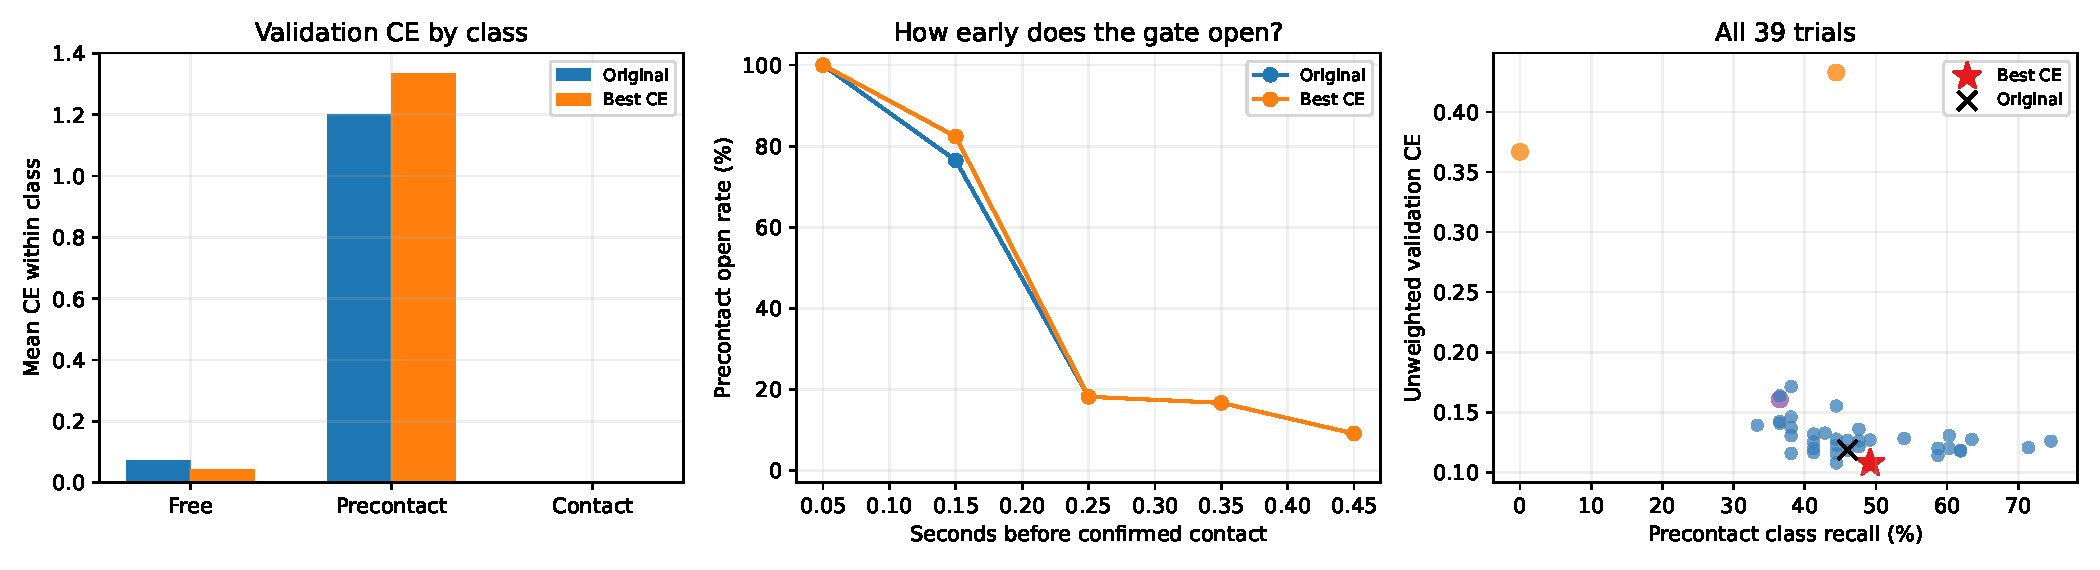
\includegraphics[width=\columnwidth]{phase_gate_analysis.pdf}
  \caption{Causal phase-gate analysis on the held-out episodes. The early
  pre-contact interval is harder than contact detection.}
  \label{fig:phase}
\end{figure}

To isolate the effect of the switch, we replaced the original phase predictor
without retraining the renderer. On 366 held-out contact/pre-contact windows,
the absolute token MSE decreased while the contact-history intervention metric
was unchanged.

\begin{table}[t]
\centering
\caption{Phase-switch replacement with a fixed renderer. The oracle uses the
offline phase reference and is an upper diagnostic, not a deployable method.}
\label{tab:phase_switch}
\setlength{\tabcolsep}{3.0pt}
\resizebox{\columnwidth}{!}{%
\begin{tabular}{@{}lrrr@{}}
\toprule
Switch & Absolute MSE & Real MSE & Response NMSE \\
\midrule
Original & 0.162983 & 0.186314 & 0.9231 \\
New causal & 0.148400 & 0.170983 & 0.9232 \\
Offline oracle & 0.082707 & 0.106732 & 0.9232 \\
\bottomrule
\end{tabular}
}
\end{table}

The switch-only result separates phase errors from the remaining image-space
response gap. It does not show that gating is superior to always-on rendering.

\subsection{Fixed-image torque intervention}
\label{sec:torque_diag}
We hold images, phase gates, and diffusion noise fixed while
replacing the complete 25-frame torque history with physical zero or a contact
history from another validation episode. The teacher's action error increases
under both interventions, showing that the teacher uses continuous torque
content. This evaluation is offline and uses the 66,000-step teacher checkpoint
from the corresponding diagnostic run.

\begin{table}[t]
\centering
\caption{Teacher action intervention on 303 held-out windows. Lower is better.
The same three diffusion seeds are paired across conditions.}
\label{tab:teacher_intervention}
\setlength{\tabcolsep}{3.8pt}
\resizebox{\columnwidth}{!}{%
\begin{tabular}{@{}lrrr@{}}
\toprule
Torque history & Raw MSE & Norm. MSE & Context change \\
\midrule
Measured & 0.010865 & 1.670325 & 0 \\
Zeroed & 0.017941 & 1.785958 & 0.408824 \\
Other-contact donor & 0.030477 & 2.496887 & 0.356835 \\
\bottomrule
\end{tabular}
}
\end{table}

For the older student readout comparison, the frozen teacher-FFN renderer has
contact response cosine $0.4770$, response NMSE $0.7868$, and student/teacher
response RMS ratio $0.3167$ for measured-minus-zero torque. The no-FFN renderer
has cosine $0.0510$ and NMSE $1.0154$. For measured-minus-other-contact torque,
the frozen-FFN renderer has cosine $0.0846$ and NMSE $1.0059$. Thus the student
transmits a reproducible coarse response to contact torque, while the specific
history-to-history response remains difficult.

\begin{figure}[t]
  \centering
  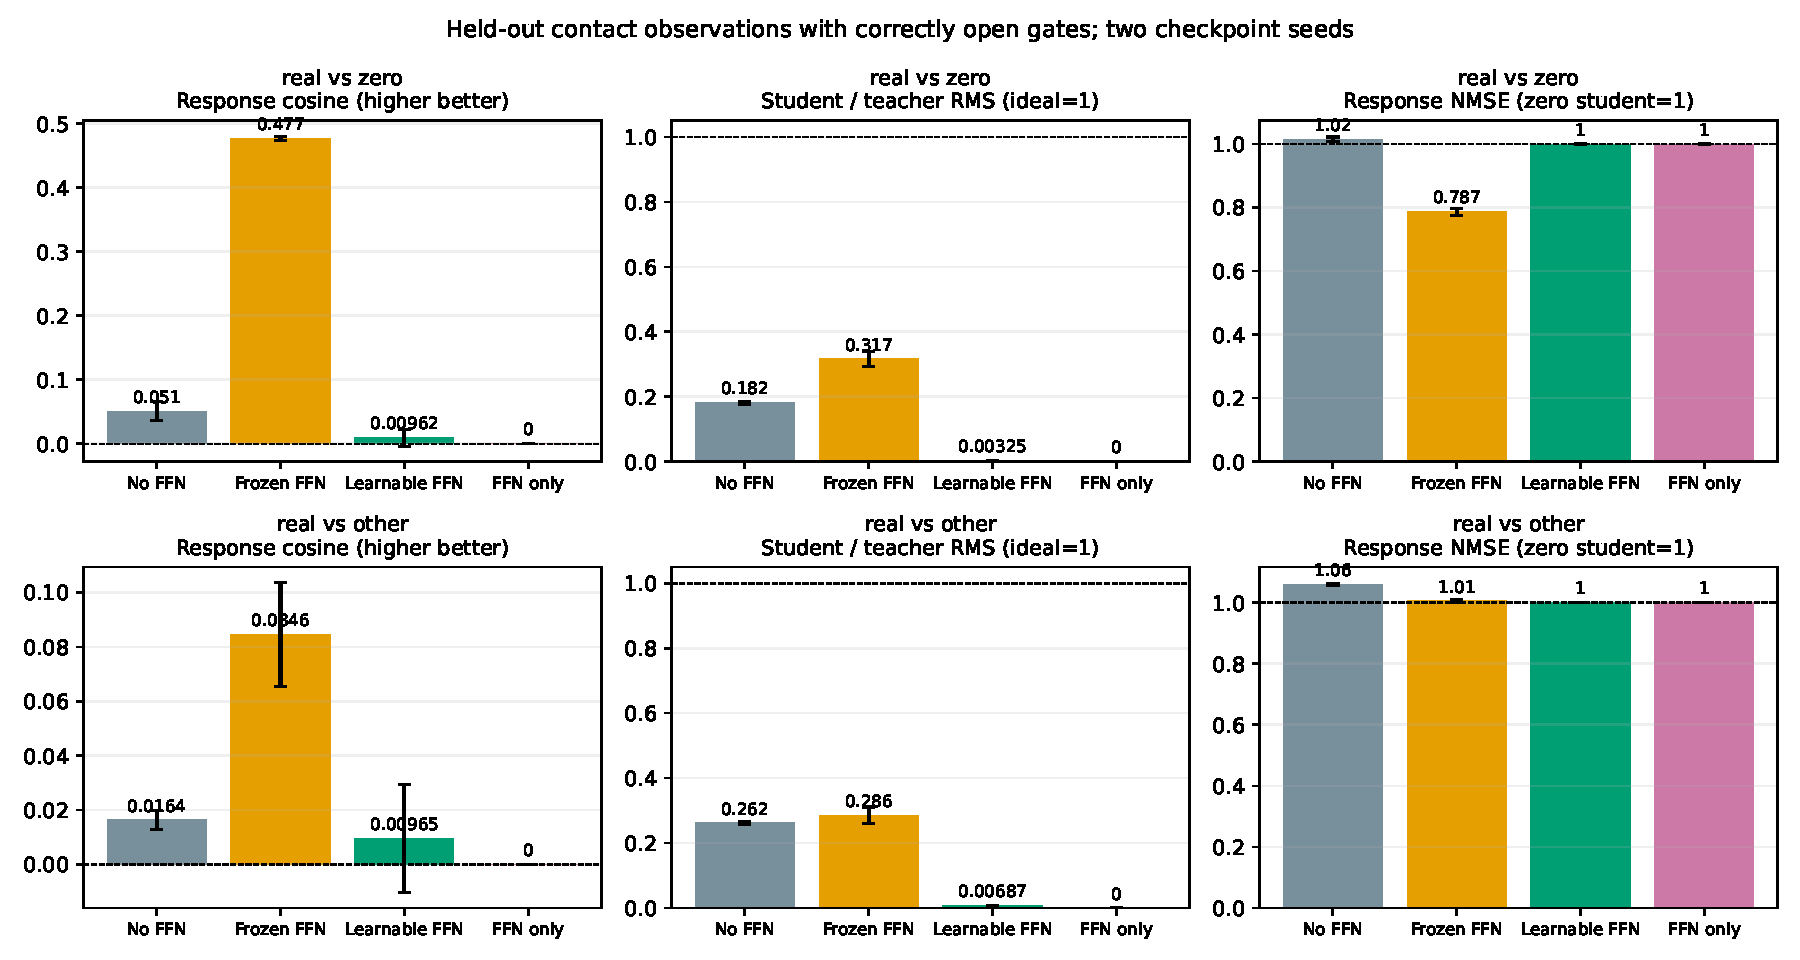
\includegraphics[width=\columnwidth]{torque_response.pdf}
  \caption{Paired torque interventions for teacher and student readouts. A
  zero-response student has NMSE one by definition.}
  \label{fig:torque_response}
\end{figure}

\subsection{Torque reliance varies across teacher checkpoints}
Figure~\ref{fig:diagnostics}(b) aggregates a separate intervention screen
across four teacher/split combinations. The plotted quantity is each
intervention's action MSE divided by that same teacher/split's measured-torque
action MSE. Images, diffusion noise, and the relevant fusion gate are held
fixed. Ratios near one indicate little action change under that intervention.

\begin{table*}[t]
\centering
\caption{Torque intervention ratios from the four-teacher diagnostic. Each
cell is action MSE divided by the same teacher/split/phase measured-torque
action MSE. The sample count is the number of phase windows.}
\label{tab:cross_teacher_torque}
\setlength{\tabcolsep}{5pt}
\begin{tabular}{@{}llrrrr@{}}
\toprule
Teacher / split & Phase ($n$) & Zeroed, gate kept & Shuffled & Fusion bypass \\
\midrule
LIBERO future F/T / train & Pre ($222$) & 4.46 & 4.68 & 2.54 \\
 & Contact ($473$) & 4.17 & 5.68 & 1.17 \\
Board blur, binary phase / held-out val & Pre ($96$) & 1.01 & 1.02 & 0.86 \\
 & Contact ($315$) & 1.04 & 1.01 & 0.85 \\
Board blur, binary phase / train & Pre ($106$) & 1.12 & 1.10 & 1.01 \\
 & Contact ($532$) & 1.14 & 1.15 & 1.06 \\
Board torque history / train & Pre ($121$) & 1.01 & 1.00 & 1.00 \\
 & Contact ($583$) & 1.27 & 1.17 & 1.00 \\
\bottomrule
\end{tabular}
\end{table*}

The LIBERO teacher shows strong sensitivity to zeroed and shuffled torque in
both pre-contact and contact. The held-out board teacher remains close to one
for zeroing and shuffling, while fusion bypass is below one in both phases.
The training-window board checkpoints show smaller effects. Since these
teacher checkpoints and data splits differ, the plot does not establish one
uniform torque-reliance level for all models. It motivates reporting the
paired intervention for the actual teacher and evaluation split associated
with each paper result.

\subsection{Readout ablation}
The short two-seed FFN study separates feature adaptation from RGB rendering.
It uses the same teacher, DINO path, phase switch, and spatial gate, with 33
held-out observations. The frozen teacher-FFN path gains from rendering, while
the independently trainable FFN can fit the teacher without becoming torque
sensitive.

\begin{table}[t]
\centering
\caption{Two-seed readout ablation. Values are mean $\pm$ population standard
deviation across the two seeds.}
\label{tab:ffn}
\setlength{\tabcolsep}{2.4pt}
\resizebox{\columnwidth}{!}{%
\begin{tabular}{@{}lrrr@{}}
\toprule
Readout & Token MSE & Open subset & RGB gain \\
\midrule
No FFN & $0.9136\!\pm\!0.0018$ & 0.8896 & 13.45\% \\
Frozen teacher FFN & $0.3602\!\pm\!0.0015$ & 0.1286 & 24.11\% \\
Trainable student FFN & $0.3449\!\pm\!0.0006$ & 0.1076 & 0.20\% \\
FFN only, no RGB & $0.3452\!\pm\!0.0016$ & 0.1080 & 0 \\
\bottomrule
\end{tabular}
}
\end{table}

\section{Additional Controls and Evidence Boundaries}
\label{sec:limits}

\subsection{Paired response-transfer study}
A separate cucumber diagnostic evaluates 303 held-out contact windows with a
frozen action head. Each donor torque history comes from another held-out
trajectory with matched contact labels. Images, predicted switch, and diffusion
noise are paired. Positive gaps mean the measured history has lower action MSE
than the donor history.

\begin{table}[t]
\centering
\caption{Response-transfer diagnostic. Raw RGB remains the strongest absolute
action readout in this offline study, while response-supervised students are
more sensitive to the correct torque history.}
\label{tab:response_transfer}
\setlength{\tabcolsep}{2.2pt}
\resizebox{\columnwidth}{!}{%
\begin{tabular}{@{}lrrrr@{}}
\toprule
Student & Measured & Donor & Gap & Positive / 303 \\
\midrule
Initial & .005995 & .005964 & $-.000030$ & 138 \\
Token MSE & .005993 & .005983 & $-.000010$ & 149 \\
Posterior & .005901 & .005942 & .000041 & 180 \\
Paired absolute & .007099 & .007696 & .000597 & 238 \\
Paired response & .006338 & .006956 & .000618 & 238 \\
\bottomrule
\end{tabular}
}
\end{table}

The response-supervised model reaches response cosine 0.229 and a student /
teacher response RMS ratio of 0.428, but its absolute action MSE remains above
the raw RGB value 0.005236. This is evidence of torque sensitivity, not a
closed-loop success claim.

\subsection{Negative controls}
Two controls delimit the representation claim. First, full-data paired
distillation on 3,873 training and 366 validation contact/pre-contact windows
does not improve absolute token error: the absolute-only endpoint has
validation MSE 0.162983, whereas the absolute-plus-response endpoint has
0.166536. The latter improves measured-minus-other-contact response NMSE from
0.9231 to 0.9146, a small single-seed change. Second, an explicit $Z^0/\Delta Z$
target renderer has validation token MSE 0.944785, compared with 0.940773 for
the current renderer. Adding 200 inverse-mapping pretraining steps gives
0.937318, only a 0.37\% improvement over the baseline under a larger budget.
These controls are retained to avoid interpreting every torque-dependent
diagnostic as a general solution to the distillation gap.

\begin{figure}[t]
  \centering
  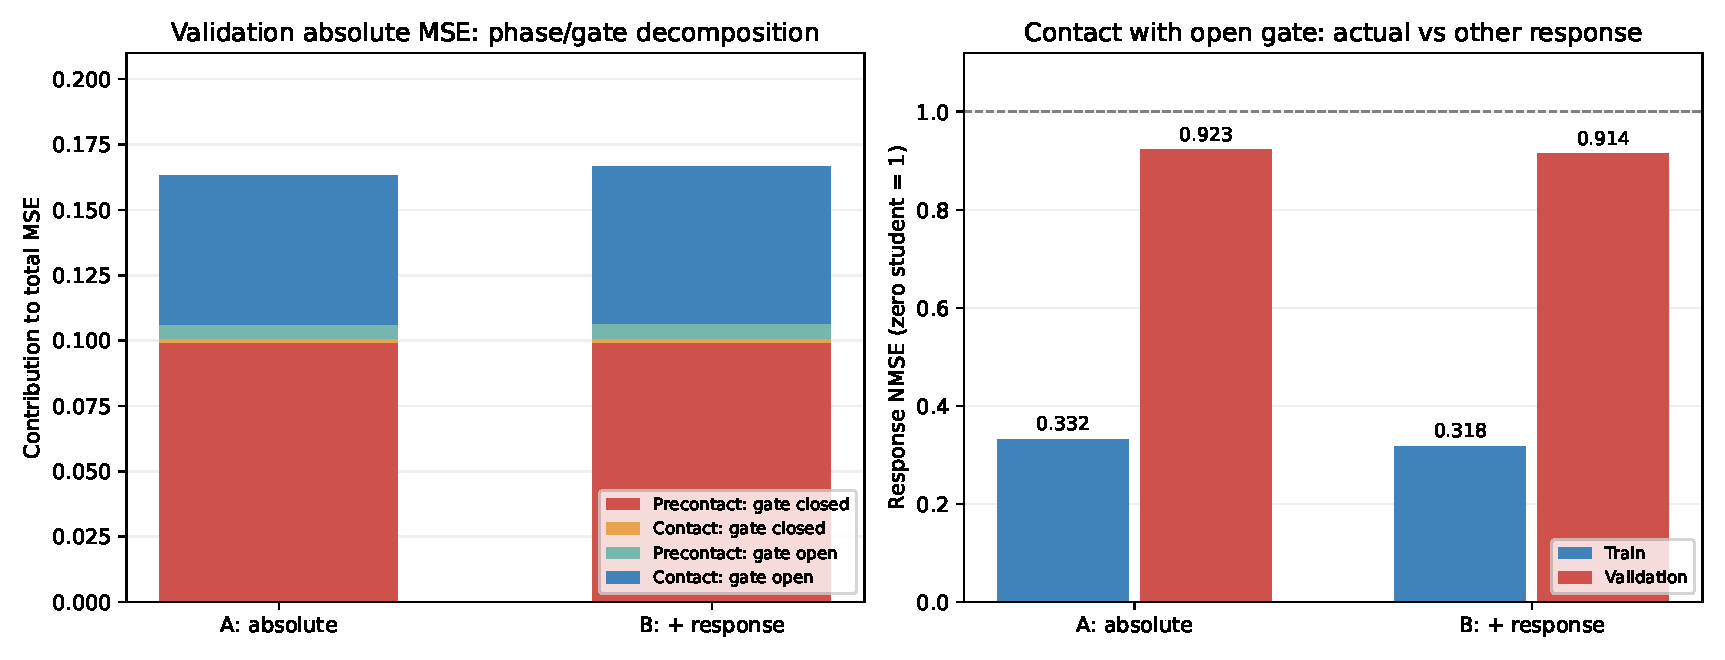
\includegraphics[width=\columnwidth]{loss_decomposition.pdf}
  \caption{Full-data paired-distillation loss decomposition. The validation
  response changes modestly while absolute error remains comparable.}
  \label{fig:loss_decomp}
\end{figure}

\subsection{Dataset splits and implementation audits}
The board distillation manifest contains 17,740 training samples and 1,893
validation samples. The six validation episodes are 5, 26, 38, 44, 53, and
60, with phase counts 1,317 free, 108 pre-contact, and 468 contact. The
cucumber response-transfer split uses 3,873 training and 366 validation
windows, with validation episodes 3, 26, and 30. Episodes are disjoint between
training and validation in both records.

The deployment audit verifies that the physical-zero path is an exact identity
when the phase switch is closed, with
\texttt{alpha0\_exact\_identity=true}, RGB
gradient norm 1.3941, and an exact same-next-update resume check. The audited
deployment renderer has 4,495,375 parameters. The phase-gate module has 4,551
parameters and its causal-history tests pass. The stage-specific token-loss
regression suite reports 72 passing tests and the DDP regression reports two
passing tests. These are engineering checks for the implementation invariants,
not additional task-success trials.

\subsection{Scope and limitations}
The main paper's real-robot evaluation consists of one 20-trial batch per method and task,
with no independent test robot or multiple training seeds. Phase references
are derived from estimated torque and are not measurements from a dedicated
force/torque sensor. The renderer is trained per task and is frozen before
downstream policy training. The intervention and response-transfer studies
are offline and use overlapping temporal windows, so their observations are
not independent repetitions. The results support a reusable RGB interface for
the evaluated tasks and policies. They do not establish universal cross-task
transfer, arbitrary-backbone equivalence, or seed robustness.

\section{Visual Evidence from Robot and Renderer Experiments}
\label{sec:visual_evidence}

\subsection{Recorded robot task sequences}
Figure~\ref{fig:task_sequences} shows representative flat- and inclined-board
wipe sequences selected from recorded robot videos. The frames illustrate the
task geometry and the progression from approach to tool contact and board
cleaning. Their phase timeline was annotated from video timestamps for the
figure and is not the deployed phase-predictor output. The sequences provide
qualitative context for the success-count comparison in
Table~\ref{tab:success}; they are not additional trials or a matched RGB/CIVI
comparison.

\begin{figure*}[t]
  \centering
  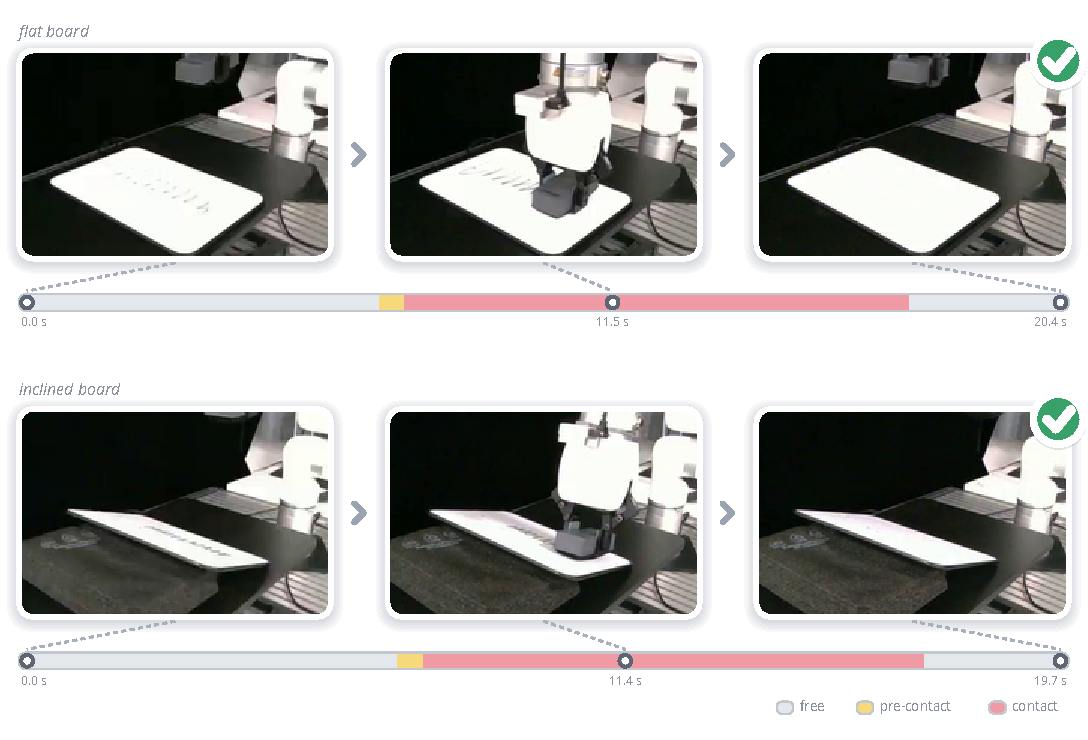
\includegraphics[width=0.96\textwidth]{task_success_examples.pdf}
  \caption{Representative recorded wipe-board sequences on flat and inclined
  boards. Frames are shown at the beginning, during the wipe, and near task
  completion. The colored phase strips are video-based annotations for this
  illustration and should not be read as phase-predictor measurements.}
  \label{fig:task_sequences}
\end{figure*}

\subsection{Spatially localized render changes}
The magnified side- and wrist-camera examples in Fig.~\ref{fig:render} show
where the renderer changes RGB. The mask in Fig.~\ref{fig:mask} is supervised
by teacher-induced visual-token changes. It is a learned representation
support, rather than an independently measured contact segmentation. These
images support the image-space mechanism described in Sec.~\ref{sec:method},
while the closed-loop results and the controlled ablations provide the
quantitative tests.

\subsection{Free, pre-contact, and contact render diagnostics}
The repository also contains a short-run renderer comparison that holds one
board sample fixed within each phase and visualizes the original image,
rendered image, and RGB residual for both side and wrist views.
Figure~\ref{fig:phase_render_grid} shows representative free, pre-contact, and
contact samples. Within each phase panel, all architecture variants receive
the same image and share its residual color scale. The displayed row uses the
interleaved-FiLM/MLP128 variant. This is a separate 1,000-update diagnostic, not the renderer checkpoint used for
the main success table. The residual panels help inspect whether the learned
transformations are spatially structured, while Table~\ref{tab:short_renderer}
reports how much the shared renderer improves over the original image under
the same feature adapter.

\begin{figure*}[t]
  \centering
  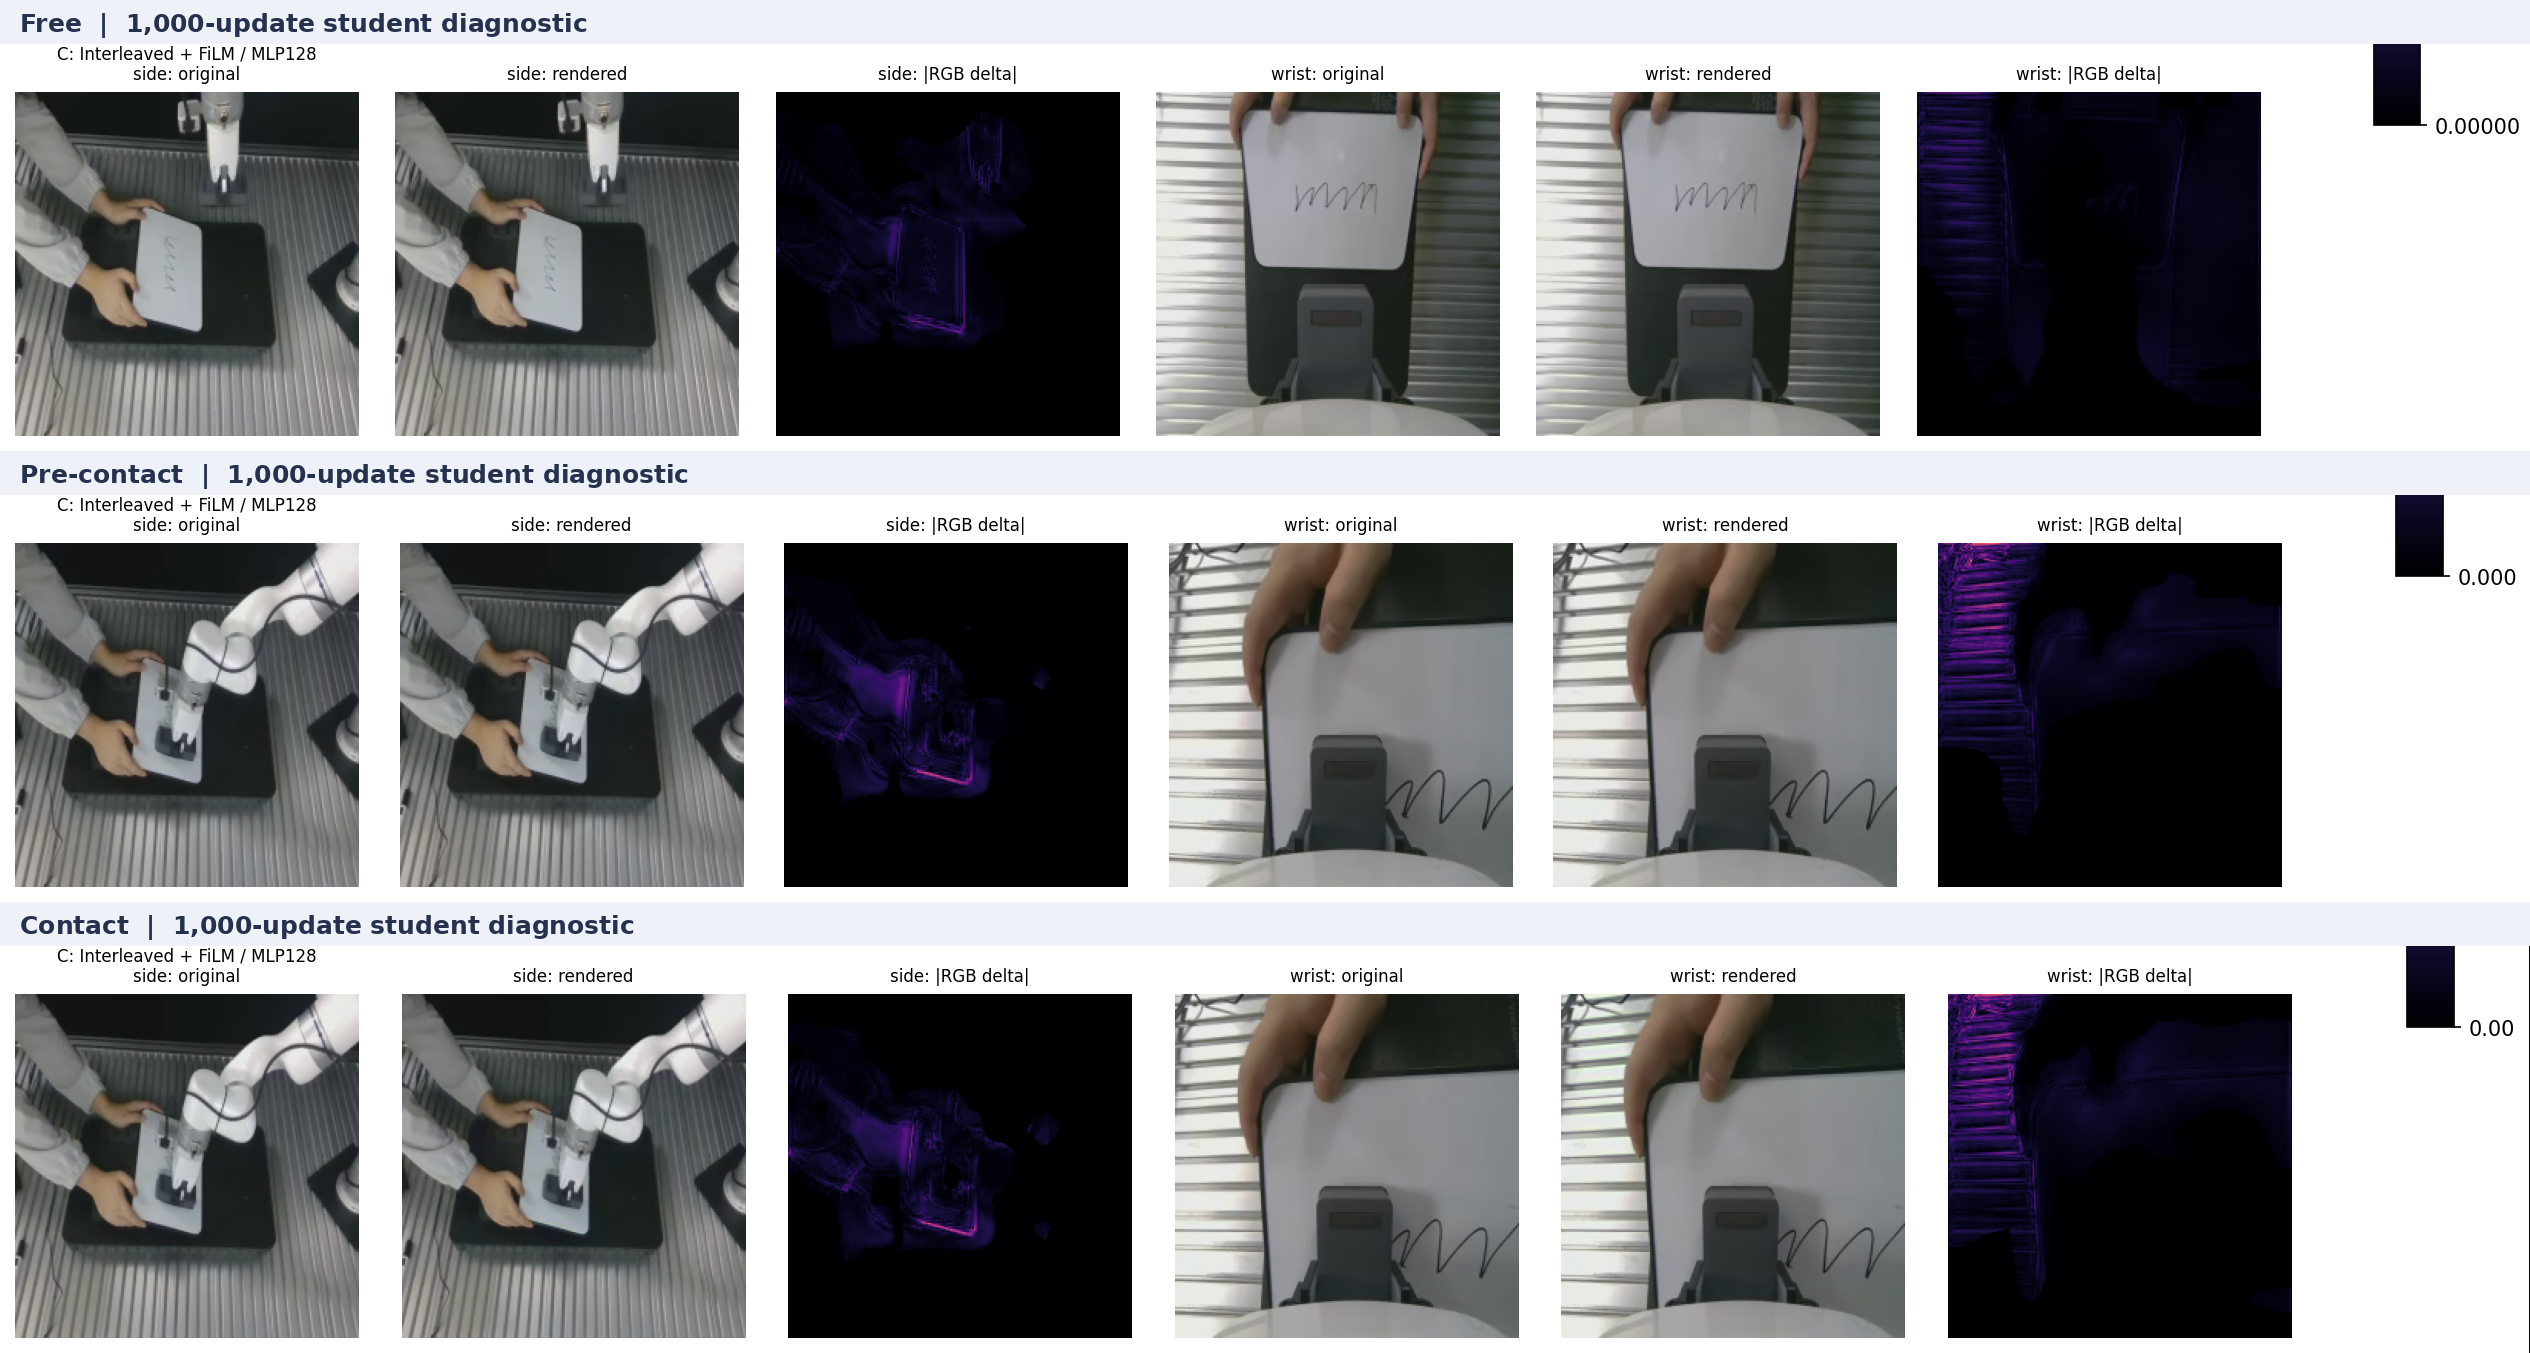
\includegraphics[width=0.96\textwidth]{phase_render_diagnostics.png}
  \caption{Additional renderer visualizations from repository experiments.
  The rows show free, pre-contact, and contact views from one fixed board sample
  with a shared RGB-residual color scale within each row. This is the
  interleaved-FiLM/MLP128 variant from the separate short-run experiment.}
  \label{fig:phase_render_grid}
\end{figure*}

\begin{table}[t]
\centering
\caption{Short-run renderer architecture comparison at the common 1,000-update
checkpoint. The last column is the renderer's improvement over original RGB
using the same frozen adapter.}
\label{tab:short_renderer}
\setlength{\tabcolsep}{2.4pt}
\resizebox{\columnwidth}{!}{%
\begin{tabular}{@{}lrrr@{}}
\toprule
Variant & Contact MSE & Response MSE & RGB gain \\
\midrule
6SA+2CA, linear & 0.173959 & 0.056424 & 1.40\% \\
2SA--CA--2SA--CA, linear & 0.174635 & 0.059519 & 1.16\% \\
Interleaved+FiLM, linear & 0.173940 & 0.058692 & 1.45\% \\
Interleaved+FiLM, MLP128 & 0.122370 & 0.048686 & 0.48\% \\
\bottomrule
\end{tabular}
}
\end{table}

The comparison uses the same teacher, phase and spatial gate, initial renderer,
loss, seed, and 1,893-window validation set. The MLP adapter lowers the
absolute feature error, but the RGB renderer adds only 0.48\% improvement over
original RGB passed through that same adapter. Its torque-response difference
MSE (0.048686) also exceeds the no-student-response reference (0.043594).
These short-run results show structured image changes, but do not establish
that the shared renderer reproduces the teacher's torque response.

\subsection{Multi-episode response visualization}
The \texttt{civi\_student\_iteration} screen includes held-out board images,
their selected RGB outputs, and RGB-RMS residual maps. Figure~\ref{fig:selected_response_visuals}
shows episodes 38 and 60 from one seed-42 checkpoint evaluated after 2,800
updates. The selected-evaluation pass performs no additional RGB updates. In a
separate two-seed comparison at 1,000 updates, realization error decreases by
6.39--6.52\% and teacher-response error by 3.07--3.11\%. Both seeds pass the
check that correct torque beats shuffled and zero torque, but neither reaches
the predeclared 25\% realization or 10\% teacher-response thresholds. The
checkpoint shown in the figure is also marked `promote=false` in the experiment
audit. These visual and numerical results show torque sensitivity while
documenting the current transfer gap.

\begin{figure*}[t]
  \centering
  \begin{subfigure}[t]{0.48\textwidth}
    \centering
    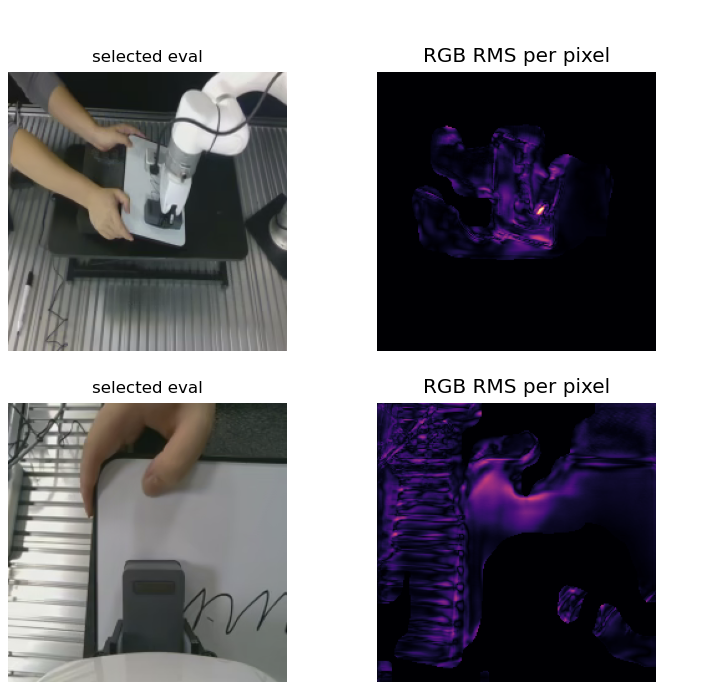
\includegraphics[width=\linewidth]{selected_rgb_ep38.png}
    \caption{Selected evaluation visualization for board episode 38.}
  \end{subfigure}
  \hfill
  \begin{subfigure}[t]{0.48\textwidth}
    \centering
    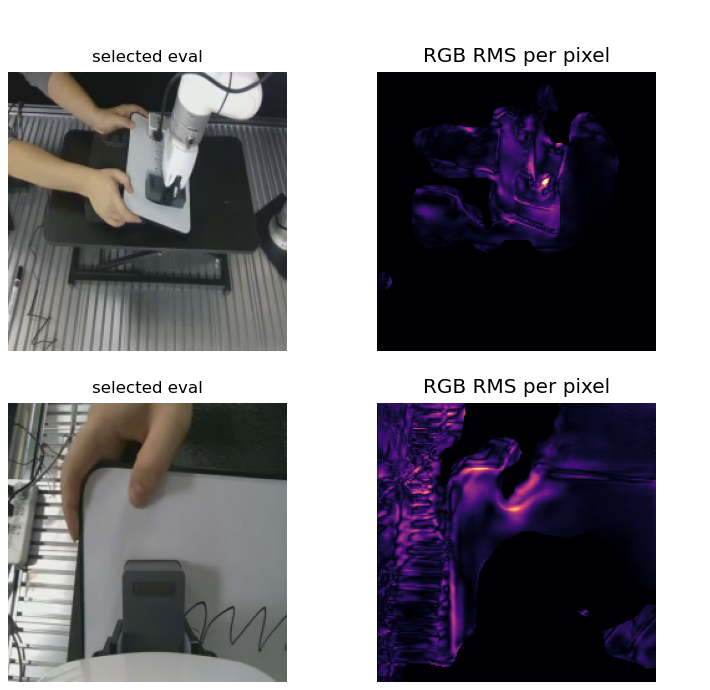
\includegraphics[width=\linewidth]{selected_rgb_ep60.png}
    \caption{Selected evaluation visualization for board episode 60.}
  \end{subfigure}
  \caption{Held-out response-decoder visualizations from the multi-episode
  student iteration screen. Each pair contains the selected RGB view and its
  RGB-RMS residual map under fixed absolute color scales.}
  \label{fig:selected_response_visuals}
\end{figure*}

\section{Phase Prediction and Gate Ablations}
\label{sec:phase_more}

\subsection{Pre-contact remains the difficult phase}
The 39-trial phase-model search reports a selected validation model and an
original baseline on the same three held-out episodes. Selection used the
validation set, so these are model-development diagnostics, not an independent
test. The selected model has lower overall CE and a slightly lower free
false-open rate, but does not improve the 0.2--0.5 second pre-contact recall.
This distinction matters for the mechanism: high overall accuracy and perfect
contact recall do not by themselves show that rendering starts early enough to
prepare for contact.

\begin{figure*}[t]
  \centering
  \begin{subfigure}[t]{0.62\textwidth}
    \centering
    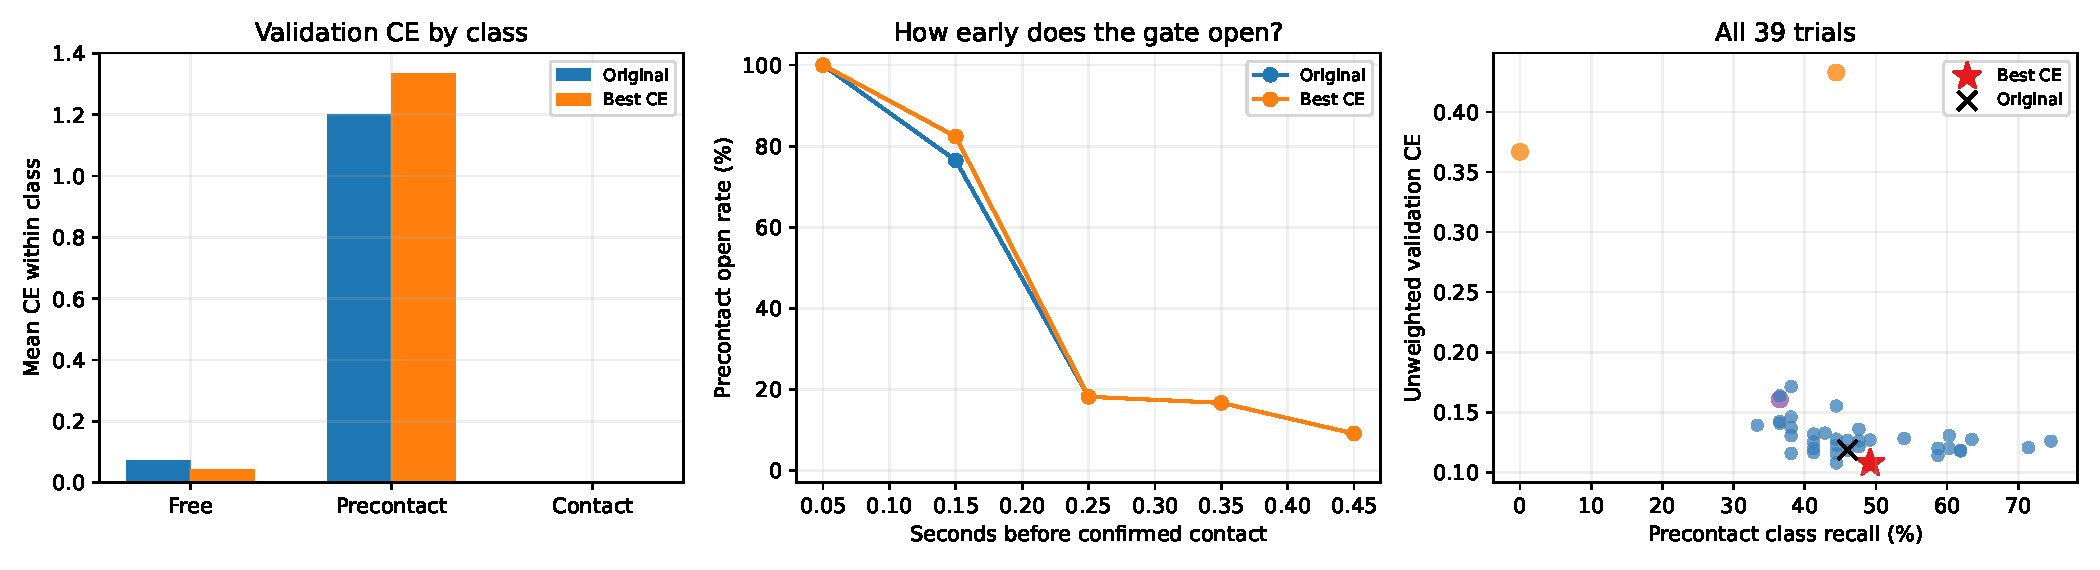
\includegraphics[width=\linewidth]{phase_gate_analysis.pdf}
    \caption{Class loss, onset-relative opening, and search trials.}
  \end{subfigure}
  \hfill
  \begin{subfigure}[t]{0.34\textwidth}
    \centering
    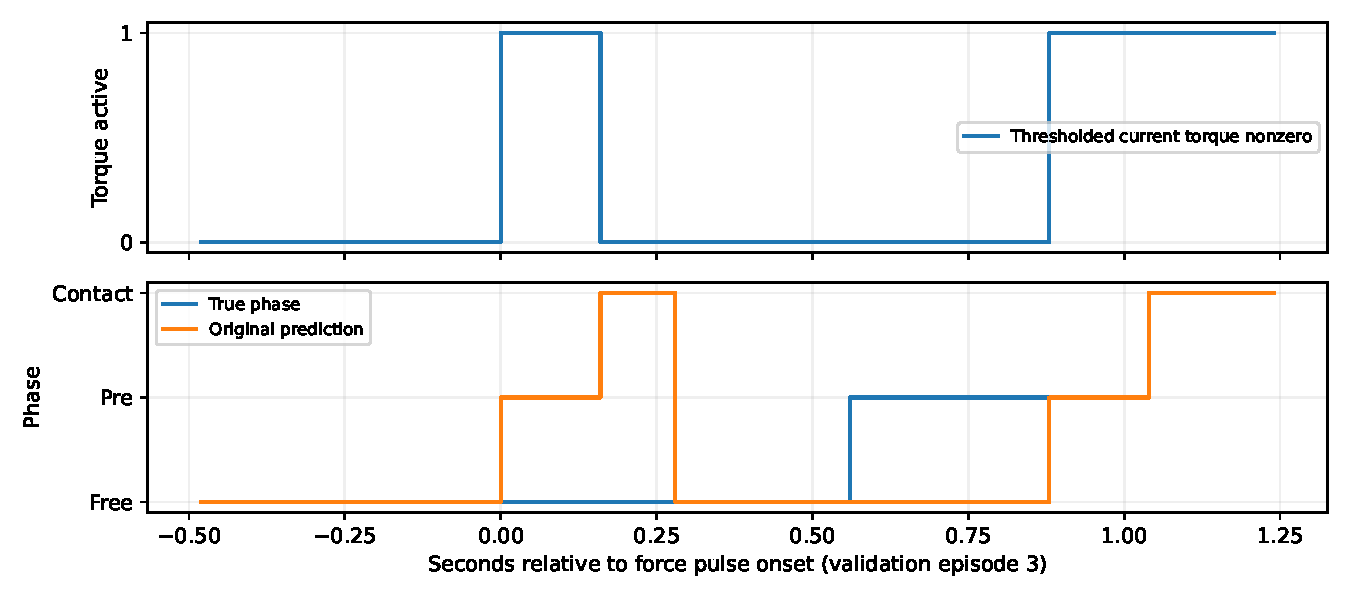
\includegraphics[width=\linewidth]{phase_false_open_event.pdf}
    \caption{One held-out pulse and phase trace.}
  \end{subfigure}
  \caption{Held-out phase diagnostics. The onset-relative plot shows that
  pre-contact prediction is concentrated near contact onset. The event trace
  illustrates one free-state false opening in the original classifier.}
  \label{fig:phase_search_more}
\end{figure*}

\begin{table}[t]
\centering
\caption{Opening rates in the same validation set. The best-CE point was
selected among 39 phase-model trials using this validation split.}
\label{tab:phase_search}
\setlength{\tabcolsep}{3pt}
\resizebox{\columnwidth}{!}{%
\begin{tabular}{@{}lrrrr@{}}
\toprule
Model & Accuracy & Free false open & Pre open & Contact open \\
\midrule
Original & 96.17\% & 0.99\% & 47.62\% & 100\% \\
Selected CE & 96.45\% & 0.85\% & 49.21\% & 100\% \\
\bottomrule
\end{tabular}
}
\end{table}

For the selected CE model, pre-contact opening is 100\% in the final 0.1
seconds before confirmed contact, 82.35\% at 0.1--0.2 seconds, and 18.18\%,
16.67\%, and 9.09\% in the successive 0.1-second bins from 0.2 to 0.5
seconds. This experiment supports a limited phase-detection claim and exposes
the difficulty of early pre-contact activation.

\subsection{Replacing the switch without retraining the renderer}
A second experiment trained a 4,551-parameter image-plus-torque GRU gate. Its
validation set contains 732 observations from three held-out episodes, including
126 pre-contact and 602 contact observations. Accuracy is 90.71\%. The gate
opens on 47.62\% of pre-contact observations and predicts the exact pre-contact
class on 46.03\%. Contact opening is 100\%, and free false-open rate is zero
on the four free observations. The small free denominator is important when
interpreting that rate.

\begin{figure*}[t]
  \centering
  \begin{subfigure}[t]{0.49\textwidth}
    \centering
    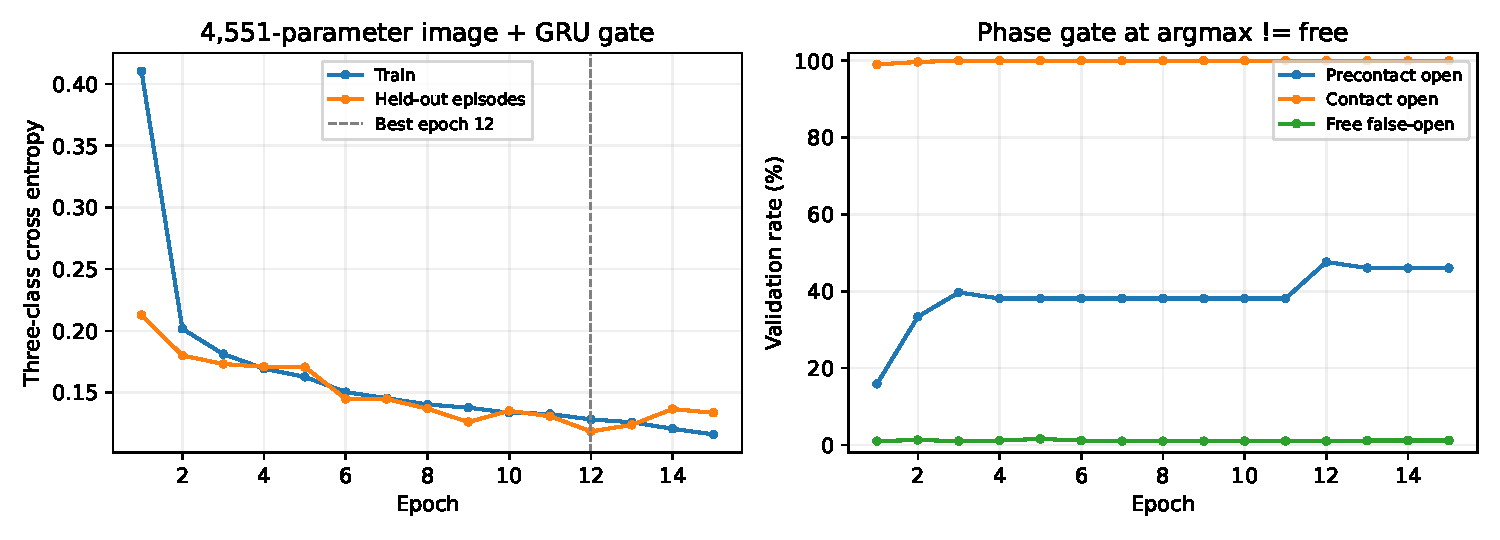
\includegraphics[width=\linewidth]{phase_gate_training.pdf}
    \caption{Image--GRU phase model training.}
  \end{subfigure}
  \hfill
  \begin{subfigure}[t]{0.49\textwidth}
    \centering
    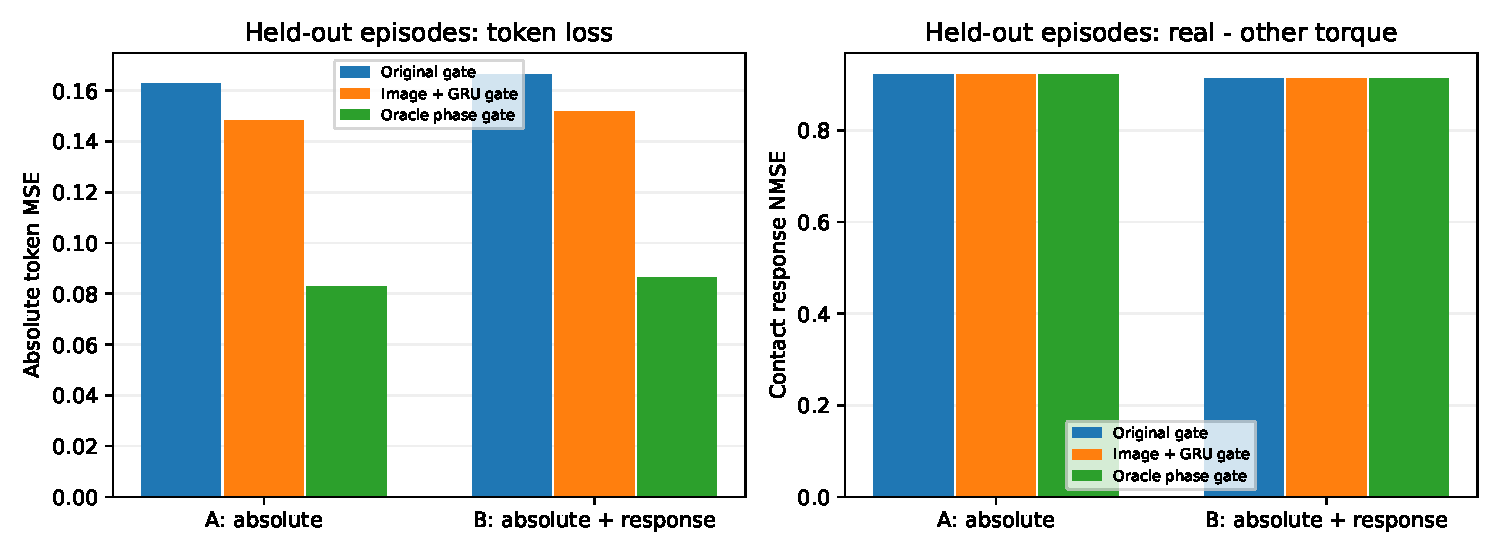
\includegraphics[width=\linewidth]{phase_gate_student_loss.pdf}
    \caption{Fixed-renderer loss under switch replacement.}
  \end{subfigure}
  \caption{Separate causal phase-gate experiment. The image--GRU gate was
  evaluated on held-out episodes. Student loss was recomputed with each gate
  while keeping renderer weights fixed.}
  \label{fig:phase_gate_replacement}
\end{figure*}

Replacing the original switch lowers absolute token MSE from 0.162983 to
0.148400 on the 366 held-out pre-contact/contact windows. The measured-minus-
other-contact response NMSE remains 0.9231 versus 0.9232. This is consistent
with a gate-related absolute-error contribution while leaving the continuous
torque-response gap unresolved. The offline phase switch reaches 0.082707
absolute MSE as an oracle diagnostic, not a deployment result.

\section{Proprioceptive Torque Signal Diagnostics}
\label{sec:torque_signal}

The paper uses sensorless external joint-torque estimates as the physical input.
The repository compares two model-based estimators, an inverse-dynamics RNEA
residual and a generalized-momentum observer, using common causal filtering on
51 erase-board episodes (21,512 frames) and 51 cucumber-peeling episodes
(22,513 frames). Figure~\ref{fig:tau_estimator} shows the seven joint
trajectories and their $\ell_1$ magnitude for one board episode.

\begin{figure*}[t]
  \centering
  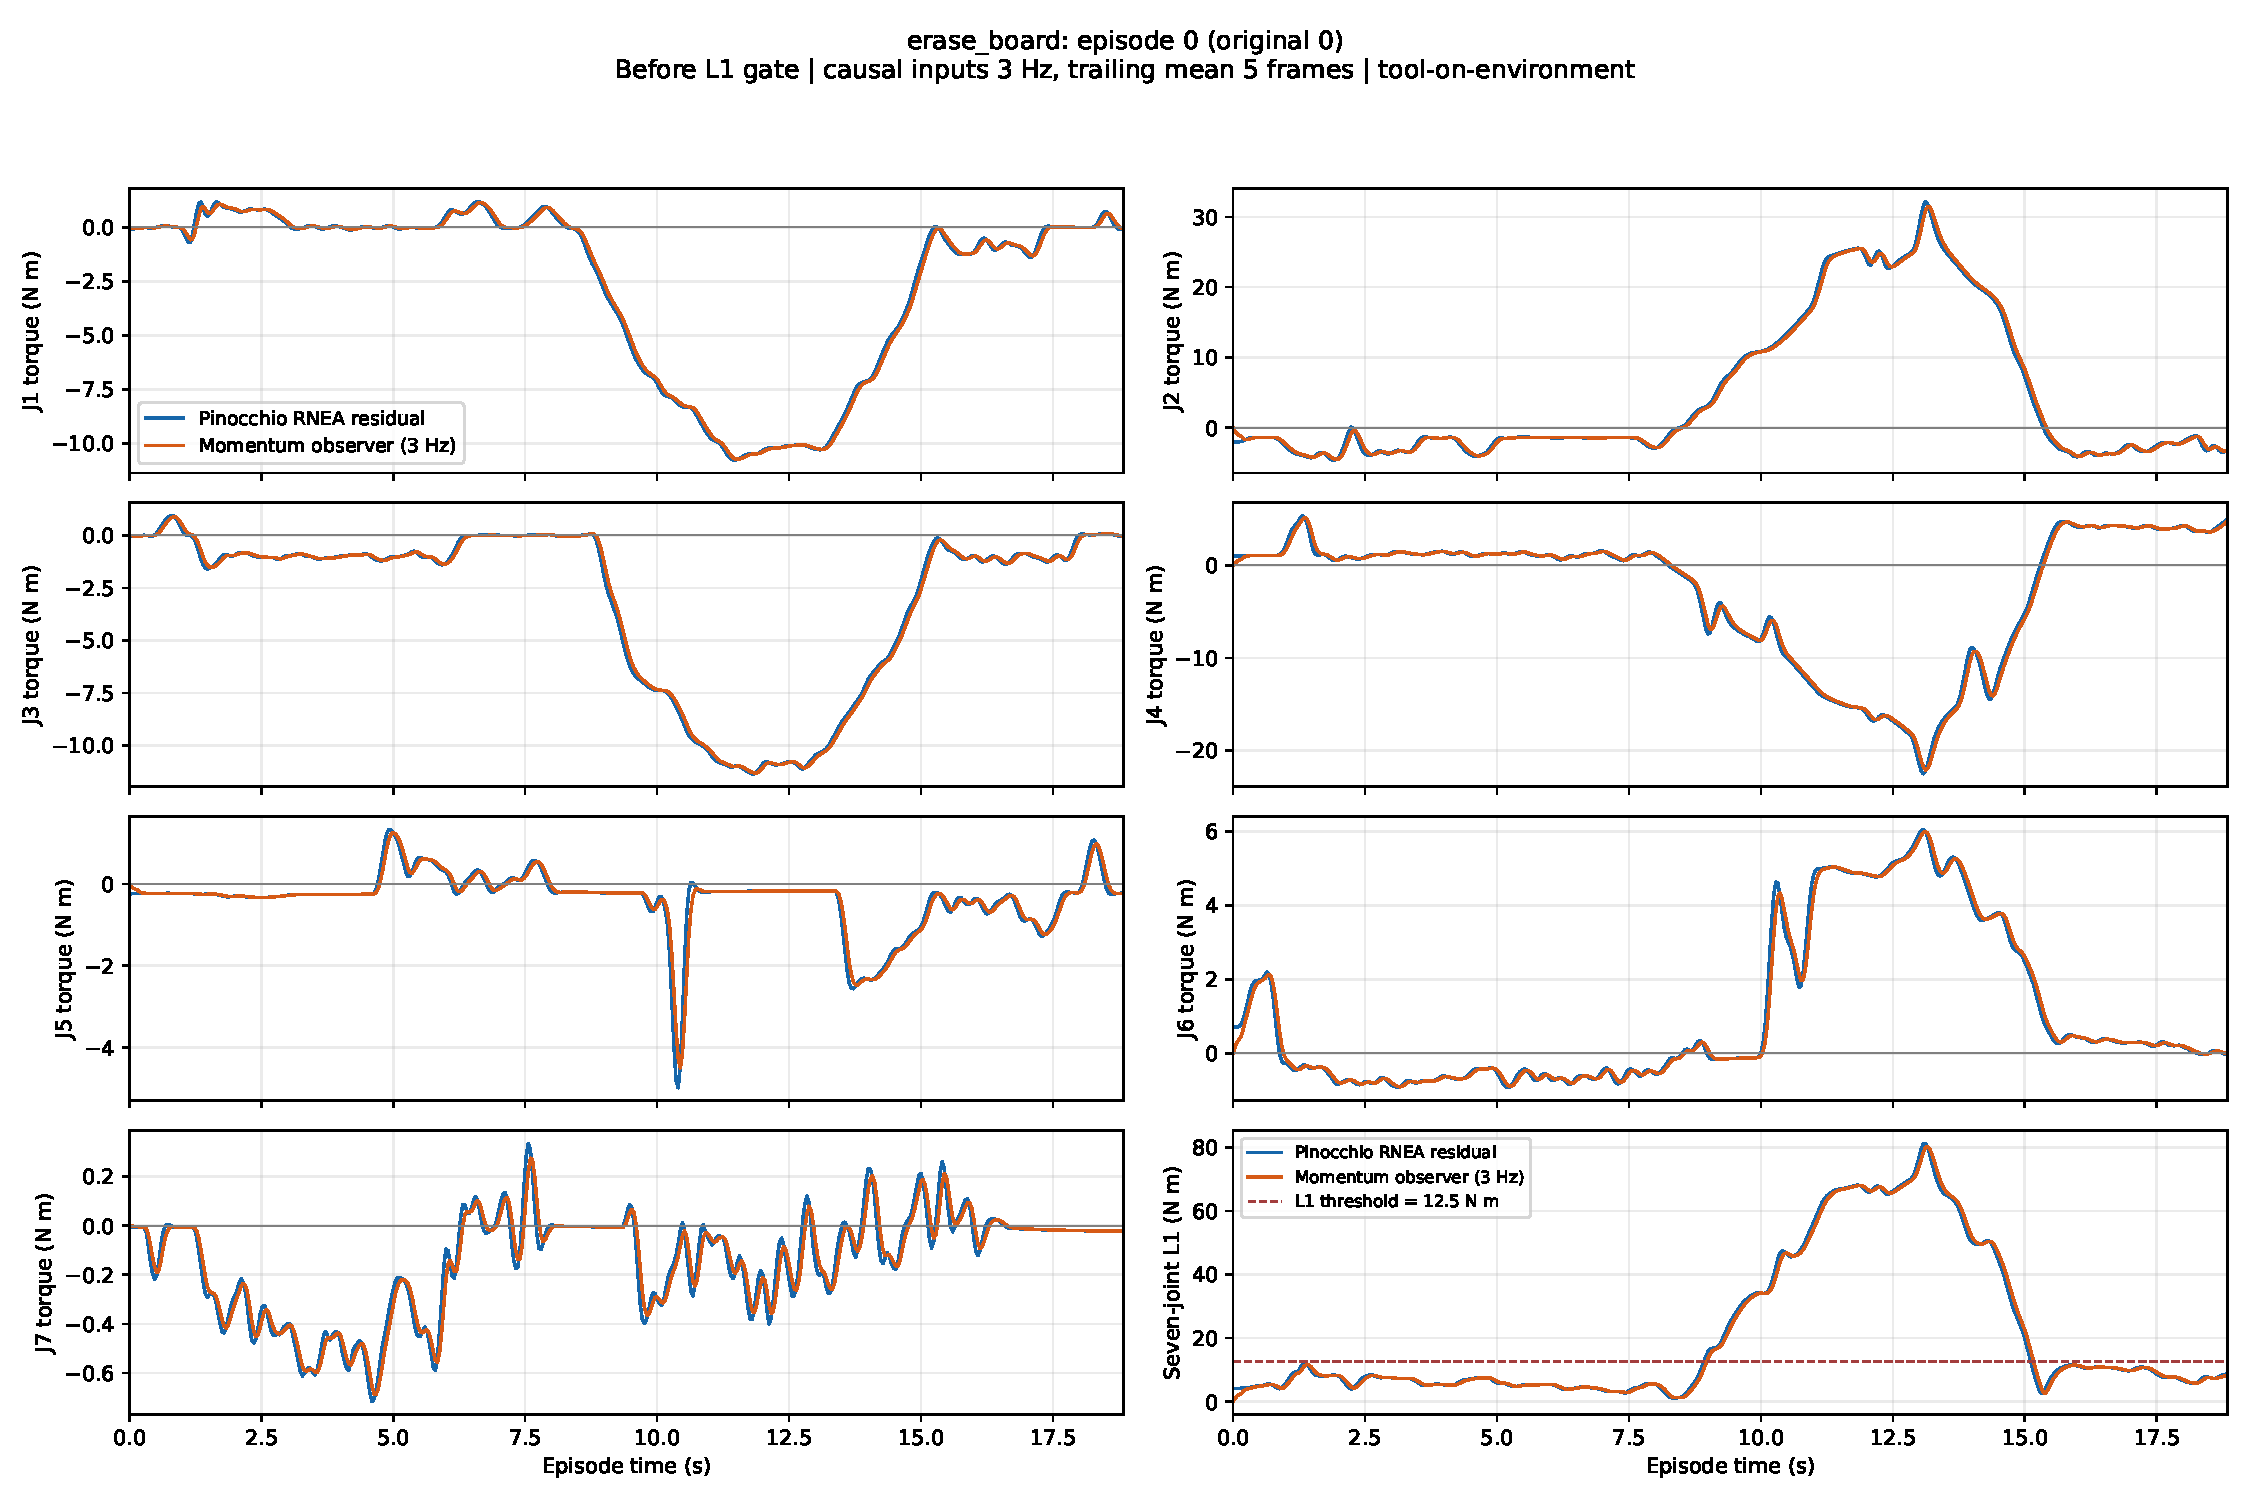
\includegraphics[width=0.94\textwidth]{board_tau_estimator_comparison.pdf}
  \caption{Two model-based external-torque estimates on one recorded wipe-board
  episode. The L1 threshold is shown for phase annotation. The comparison does
  not use an external force/torque sensor as ground truth.}
  \label{fig:tau_estimator}
\end{figure*}

\begin{table}[t]
\centering
\caption{Episode-0 torque-estimator summary. Both methods use the same 3-Hz
causal input filtering, trailing five-frame smoothing, and 12.5-Nm L1 threshold.}
\label{tab:tau_estimator}
\setlength{\tabcolsep}{3.4pt}
\resizebox{\columnwidth}{!}{%
\begin{tabular}{@{}llrrr@{}}
\toprule
Task & Estimate & Mean L1 & Max L1 & Above threshold \\
\midrule
Erase board & RNEA & 21.14 & 81.29 & 32.84\% \\
 & Momentum observer & 21.07 & 80.33 & 32.84\% \\
Peel cucumber & RNEA & 12.08 & 36.22 & 34.17\% \\
 & Momentum observer & 11.99 & 35.99 & 33.49\% \\
\bottomrule
\end{tabular}
}
\end{table}

Both estimates agree closely after shared filtering on these episodes. This is
a consistency check between two dynamics-based estimates, not a measurement of
sensor accuracy. The estimator study also reports uncalibrated friction,
torque-bias, and payload assumptions, so we retain the limitation that torque
quality can affect the interface.

\section{Additional Paired-Response and Image-Space Experiments}
\label{sec:paired_extra}

\subsection{Paired student action readout}
The 303-window cucumber study pairs the image, phase switch, and diffusion noise
while replacing measured torque with matched contact histories from other
held-out episodes. It uses the same frozen action head for raw RGB and all
rendered variants. Figure~\ref{fig:paired_learning} plots training trajectories
and held-out action error. Response-supervised rendering makes the action
readout more sensitive to correct versus donor torque, but the raw RGB
condition still has the lowest absolute action MSE in this offline test.

\begin{figure}[t]
  \centering
  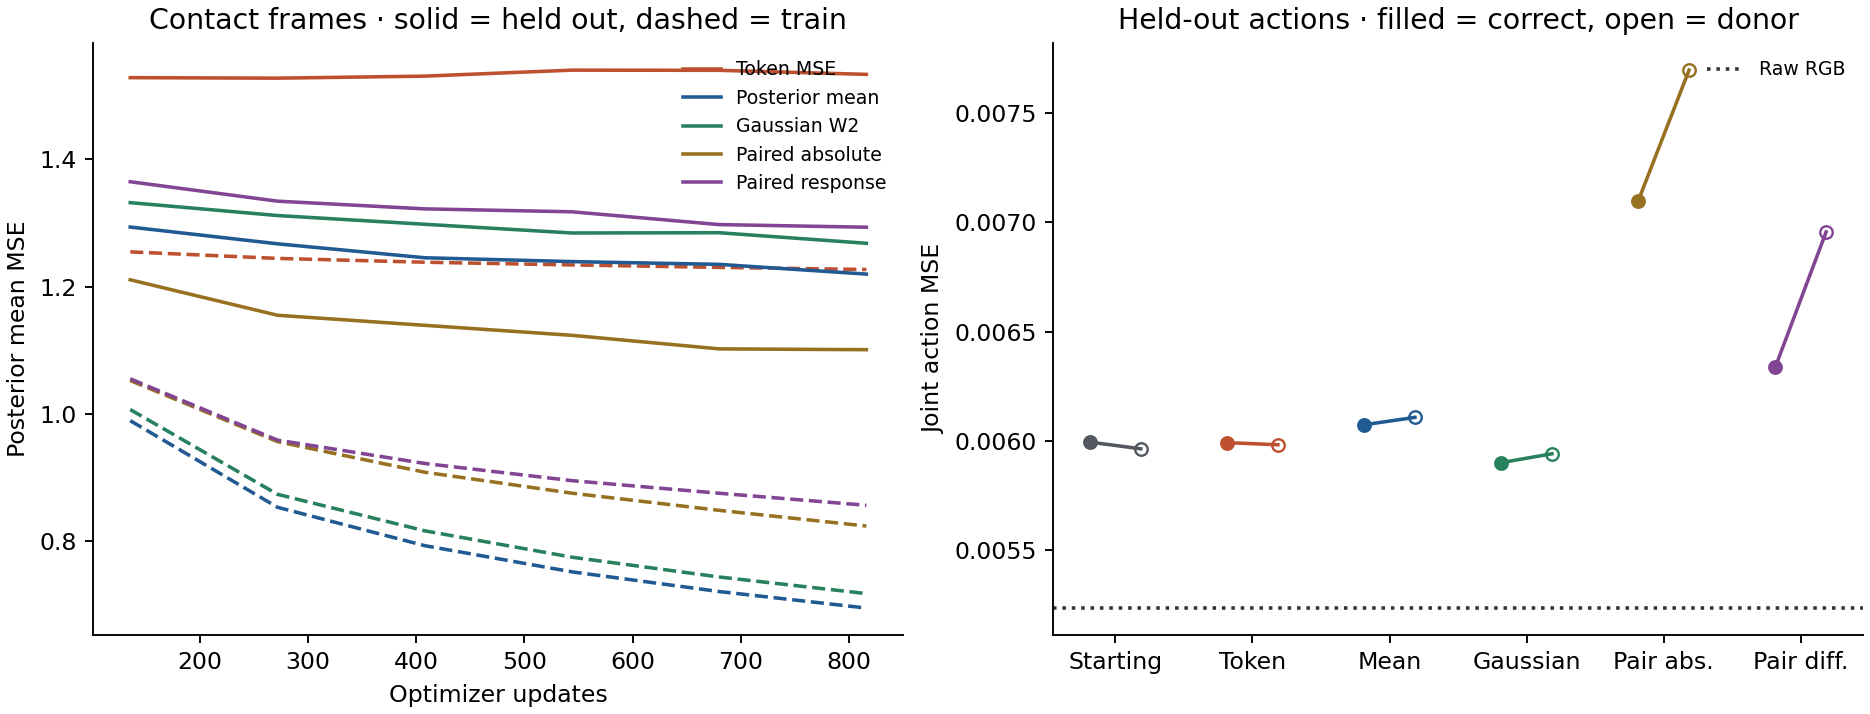
\includegraphics[width=\columnwidth]{paired_response_learning.png}
  \caption{Cucumber paired-response experiment. Left: posterior-mean feature
  error during training. Right: held-out action MSE for measured and donor
  torque histories, using paired diffusion noise and the same frozen action
  head.}
  \label{fig:paired_learning}
\end{figure}

The response-target student yields 0.006338 action MSE with measured torque and
0.006956 with donor torque, a paired gap of 0.000618. The same student's
response cosine to the teacher is 0.229 and response RMS ratio is 0.428.
However, its absolute action MSE is higher than raw RGB at 0.005236, and the
validation set comprises only three independent trajectories with overlapping
windows. We interpret this as offline evidence that the rendered input can
carry torque-dependent action information, not as a task-success improvement.

\subsection{Per-window RGB optimization as a reachability diagnostic}
The short renderer diagnostic also optimizes RGB independently for each of 12
fixed held-out windows. With 200 per-window updates, the gated pixel solution
reduces contact-token MSE by 56.4\% relative to its zero-residual starting
point. The shared renderer trained for 1,000 updates only improves the matched
objective by 0.48\% over original RGB with the same frozen MLP adapter.

\begin{table}[t]
\centering
\caption{Per-window image optimization diagnostic. The per-window solution
uses each evaluated image directly and is an offline upper diagnostic, not a
deployable renderer.}
\label{tab:reachability}
\setlength{\tabcolsep}{3.2pt}
\resizebox{\columnwidth}{!}{%
\begin{tabular}{@{}lrr@{}}
\toprule
Condition & Contact token MSE & Budget \\
\midrule
Original RGB + frozen MLP & 0.119342 & shared readout \\
Shared RenderNet + frozen MLP & 0.118928 & 1,000 updates \\
Gated per-window RGB fit & 0.051978 & 200/window \\
\bottomrule
\end{tabular}
}
\end{table}

The per-window solution is optimized separately on each displayed image, so it
does not test image generalization. It shows that some token-space changes can
be reached through RGB under the diagnostic constraints, while the short-run
shared network fails to realize most of that per-image fit. It is not a
mathematical lower bound and does not establish that the paper's longer-trained
renderer has the same limitation.

\begin{figure}[t]
  \centering
  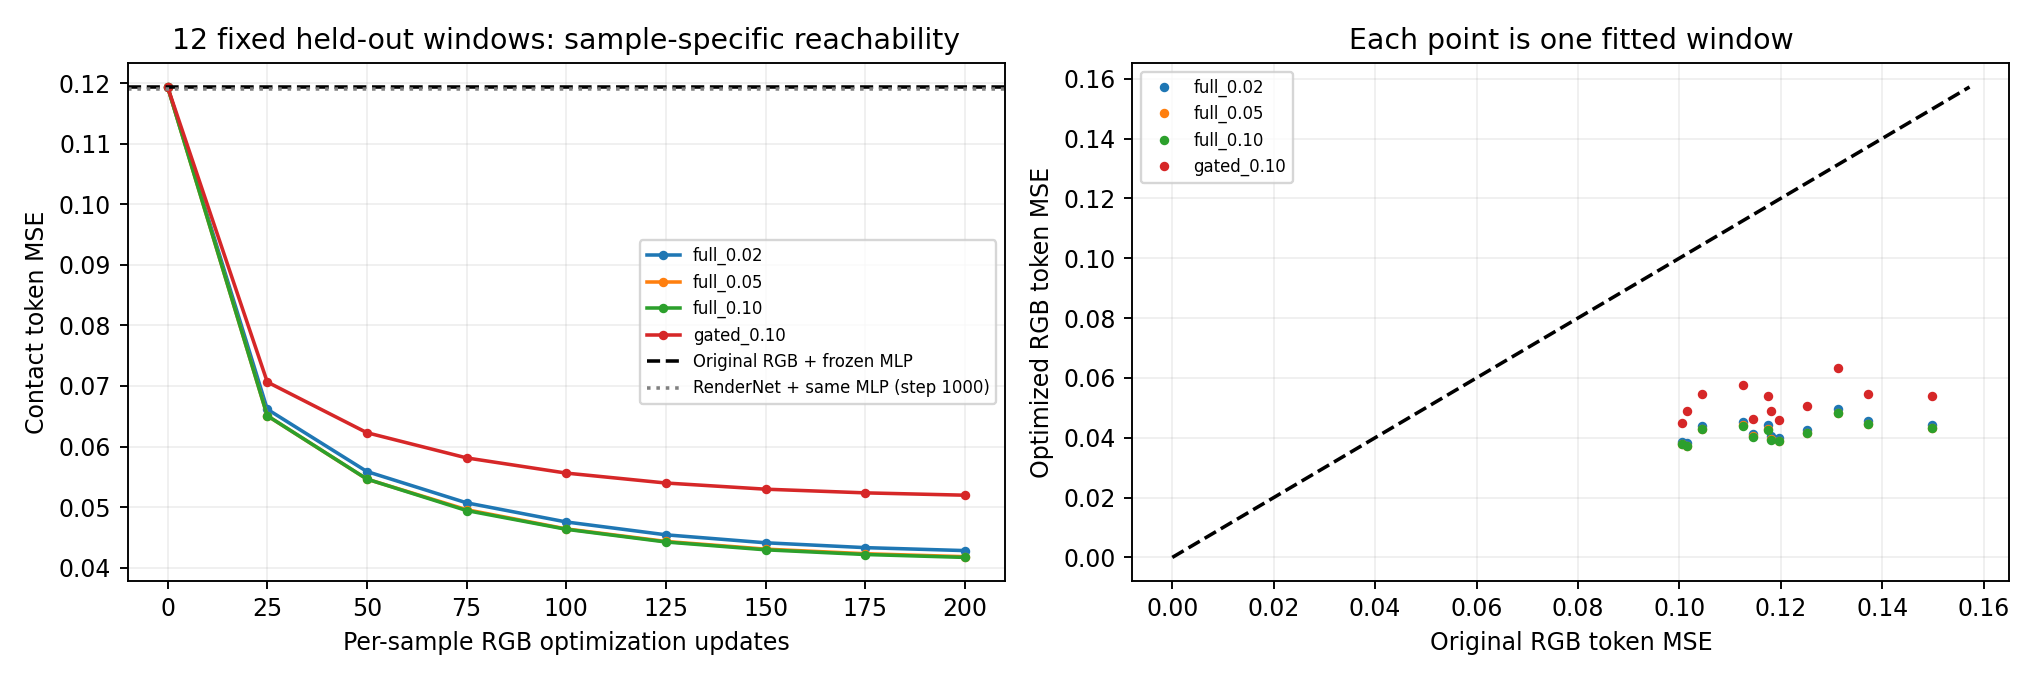
\includegraphics[width=\columnwidth]{rgb_reachability.png}
  \caption{Per-window contact-token MSE under constrained pixel optimization.
  These are 12 fixed samples, each optimized independently.}
  \label{fig:rgb_reachability}
\end{figure}

\section{Attention and Context in Teacher Fusion}
\label{sec:fusion_probes}

\subsection{What does an attention map measure?}
The teacher in Sec.~3.2 of the paper uses image patches as queries. For
patch $p$, a cross-attention weight $a_{pk}$ measures the share given to
encoded torque state $k$, with $\sum_k a_{pk}=1$. The weights alone omit
the value vectors, the output projection, the phase switch and the
subsequent feed-forward and normalization layers. To see their combined
effect, we compare the final context of the same image under the recorded
signal $W$ and a raw-zero input $W_0$, patch by patch:
\begin{equation}
 d_p=\|Z_p(I,W)-Z_p(I,W_0)\|_2 .
 \label{eq:paired_context}
\end{equation}
In this replay, zeroing also recomputes the signal-dependent switch. The
fixed-switch experiment below isolates the effect of torque content.

\begin{figure*}[t]
  \centering
  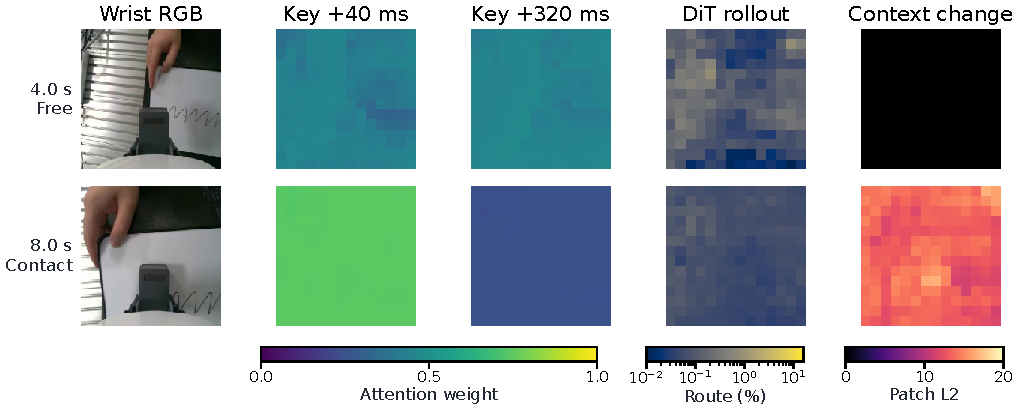
\includegraphics[width=.90\textwidth]{board_attention_context.pdf}
  \caption{Attention and context on the same real-board wrist observation.
  Rows show episode 0 at 4.0 and 8.0\,s. Columns from left show RGB, two of
  eight pre-gate cross-attention weights (four-head mean), action-to-image
  attention rollout, and the final raw-zero context distance in
  Eq.~\ref{eq:paired_context}. Both rows use the same scale in each column.
  The rollout scale is logarithmic, in percent of all routed conditioning
  mass per patch. The maps use the latest observation of the two-frame input.
  This archived 100k-step teacher uses privileged future torque.}
  \label{fig:board_attention_context}
\end{figure*}

Figure~\ref{fig:board_attention_context} uses a one-block diagnostic teacher
with eight torque keys at offsets of $+40$ to $+320$\,ms. During free motion
the first and last keys receive mean wrist-patch weights of 0.427 and 0.449.
The switch is closed and every wrist patch has $d_p=0$. During contact the
two weights are 0.747 and 0.248, and the mean wrist $d_p$ is 13.52 in
feature units. Thus a nonzero attention weight can coexist with exact visual
bypass. The rollout traces the executed action queries through eight decoder
layers and averages eight denoising calls. It uses equal residual weighting
and assumes a 50/50 image--torque split when fusion is open. Its spatial
pattern describes that routing assumption. A change in action requires an
intervention such as the one in Table~\ref{tab:teacher_intervention}.

\subsection{Matched fusion architectures on real-board data}
We trained three two-block teachers from common initialization for 5,000
updates each. All use a frozen DINOv3 encoder, a two-layer torque LSTM and
the same diffusion action head. The first teacher applies residual
cross-attention (CA). The second pools the eight torque tokens and uses
FiLM to scale and shift image features in each block. The third adds
residual FiLM after each CA and feed-forward block. The training set
contains 6,175 windows from 20 episodes. Seed 42, batch size 16, the blur
schedule, training order and evaluation noise are shared. We evaluate the
final EMA weights on clear images from episodes 5, 26, 39, 45 and 61.

\begin{figure*}[t]
  \centering
  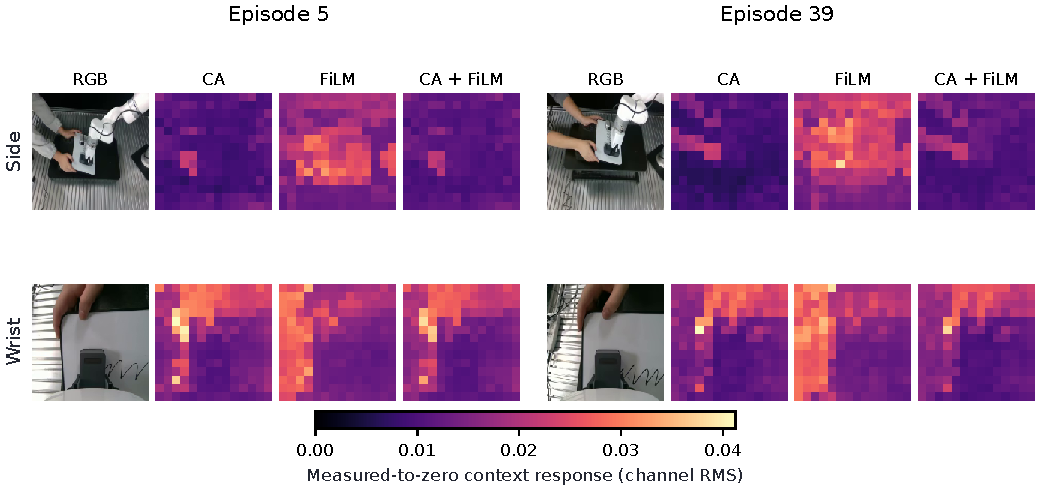
\includegraphics[width=.96\textwidth]{fusion_architectures.pdf}
  \caption{Where torque changes the teacher context on real-board data.
  The RGB and three response maps in each group refer to the same
  observation. We show the first archived contact probe in episodes 5 and
  39, for both cameras, using the latest observation. Color is the RMS
  across feature channels of the measured-minus-zero token difference,
  with the original phase gate fixed and one scale for all twelve maps.
  FiLM spreads the side-view response over more patches in these examples.
  The pooled results for all five episodes appear in
  Table~\ref{tab:fusion_operators}.}
  \label{fig:fusion_architectures}
\end{figure*}

\begin{table*}[t]
  \centering
  \caption{Matched real-board teacher ablation at 5,000 updates. Context RMS
  compares measured and physical-zero torque at fixed phase over both input
  times, both cameras and all channels. Action MSE uses original action
  units and paired eight-step DDIM sampling. Shuffling uses another window
  of the same phase without self-pairs. Columns count windows, with phase
  defined at the final observation.}
  \label{tab:fusion_operators}
  \setlength{\tabcolsep}{5pt}
  \begin{tabular}{@{}lrrrrrrr@{}}
  \toprule
  & \multicolumn{4}{c}{Measured-to-zero context RMS}
  & \multicolumn{3}{c}{Action MSE $\downarrow$} \\
  \cmidrule(lr){2-5}\cmidrule(l){6-8}
  Teacher & Free (1,136) & Pre (96) & Contact (315) & All (1,547)
    & All & Contact & Contact, shuffled \\
  \midrule
  Residual CA & .00313 & .01774 & .06129 & .02813 & .015981 & .014706 & .014883 \\
  FiLM only   & .00177 & .01180 & .04724 & .02157 & .015582 & .014060 & .014241 \\
  CA + FiLM   & .00299 & .01771 & .06103 & .02801 & .015972 & .014602 & .014815 \\
  \bottomrule
  \end{tabular}
\end{table*}

Figure~\ref{fig:fusion_architectures} and Table~\ref{tab:fusion_operators}
address two different design questions. CA has the largest contact response
RMS (0.06129). FiLM-only has a smaller response (0.04724) and the lowest
contact action MSE (0.014060), 4.4\% below CA. FiLM-only retains a
similar advantage under shuffled torque, so this error difference cannot
be attributed wholly to better use of the matched history. Adding FiLM
to CA changes overall action MSE from 0.015981 to 0.015972. Under this
training budget, the extra modulation yields little additional action
accuracy. The five episodes share one training seed. Free-anchor windows
can include a preceding active observation, which explains their small
nonzero pooled RMS.

\section{Simulation and Real-Robot Training Results}
\label{sec:sim_real}

\subsection{Paired context changes over an episode}
Figure~\ref{fig:sim_real_context} follows Eq.~\ref{eq:paired_context}
through two recorded episodes. On the simulated drawer-and-bowl task,
we replay the same RGB and six-axis wrench through the base teacher and
a variant with a CNN applied to a central high-resolution wrist crop.
Both read eight future wrench samples ($+50$ to $+400$\,ms).
At 3.0\,s, the mean wrist-patch change is 6.23 for the base checkpoint
and 2.87 for the crop checkpoint. Across the whole episode both respond
around the same contact intervals. The checkpoints were saved at 180k
and 60k steps, respectively, so the difference includes training budget
as well as architecture.

\begin{figure*}[t]
  \centering
  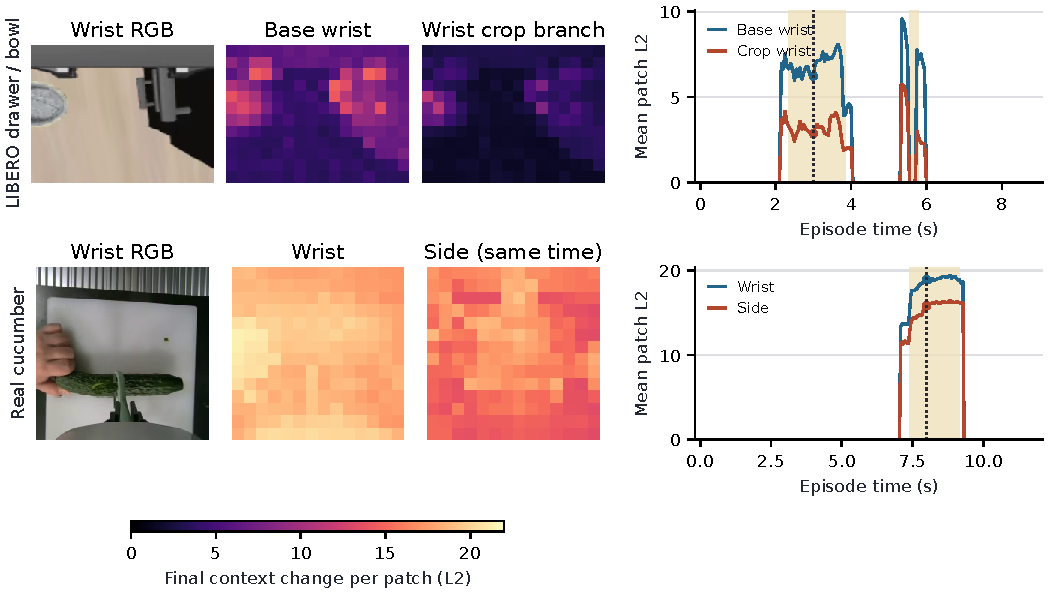
\includegraphics[width=.96\textwidth]{sim_real_context.pdf}
  \caption{Final context sensitivity over time in simulation and on a real
  robot. Top: two simulated drawer-and-bowl teachers on episode 0,
  wrist view at 3.0\,s (anchor 60). Bottom: one real-cucumber
  teacher on episode 0, wrist and side views at 8.0\,s (anchor 200).
  Spatial maps show per-patch feature L2 under raw-zero replay. Lines
  average patches of the latest observation at every anchor. Shading
  marks recorded-signal contact intervals and dots mark the images shown.
  The models learn distinct feature spaces. Absolute magnitudes describe
  each checkpoint's own response.}
  \label{fig:sim_real_context}
\end{figure*}

The cucumber teacher instead encodes 50 measured joint-torque samples at
25\,Hz and uses two CA blocks. The wrist and side views at 8.0\,s have
mean patch distances of 18.92 and 15.84. Both curves increase near
contact with the cucumber and return to zero later in the episode. This
is the 66k-step binary-phase teacher. The separate contact-only teacher
in Table~\ref{tab:teacher_intervention} also has 66k updates but takes
a 25-frame history and holds its gate fixed for the intervention.

\subsection{How much of the context gap reaches RGB?}
Table~\ref{tab:alignment_domains} gives the recorded student validation
errors. We select the epoch with minimum all-token MSE in each run and
compare it with the first validation epoch of that run. The LIBERO
reference starts with a frozen, zero RGB residual, and uses 945 student
validation windows from episodes 4, 21, 31, 36 and 49. The teacher for
this run trained on all 50 demonstration episodes. The two board
students use causal torque histories and a predicted switch. Their
open-token population can change across epochs. These denominators
matter when interpreting the different percentage reductions.

\begin{table*}[t]
  \centering
  \caption{Offline RGB distillation on simulated and recorded real data.
  Each pair gives context-token MSE at the first validation epoch and at
  the epoch selected by all-token MSE. The last column is computed within
  each run as $100(1-\mathrm{selected}/\mathrm{first})$ for open tokens.}
  \label{tab:alignment_domains}
  \setlength{\tabcolsep}{3pt}
  \small
  \begin{tabular}{@{}llrrrr@{}}
  \toprule
  Data & Teacher / gate target & Epoch & All tokens & Open tokens & Reduction \\
  \midrule
  LIBERO drawer / bowl & Future F/T & 133 & $.19226\to.08892$ & $.60377\to.27825$ & 53.9\% \\
  Real board & Blur-trained, binary phase & 35 & $.22903\to.19480$ & $.75149\to.59343$ & 21.0\% \\
  Real board & Eight-frame torque threshold & 37 & $.19843\to.14076$ & $.81575\to.57372$ & 29.7\% \\
  \bottomrule
  \end{tabular}
\end{table*}

A complementary intervention bypasses only the decoder's spatial
modulation layers in each frozen student. Figure~\ref{fig:decoder_modulation}
shows when this choice affects the output pixels. Over episode 0, pooled
RGB RMSE between the two renders is 0.02616 in LIBERO and 0.01357 on
the board, for RGB values in $[0,1]$. The downstream error comparison
for the main robot tasks is given in Table~\ref{tab:ablation}.

\begin{figure}[t]
  \centering
  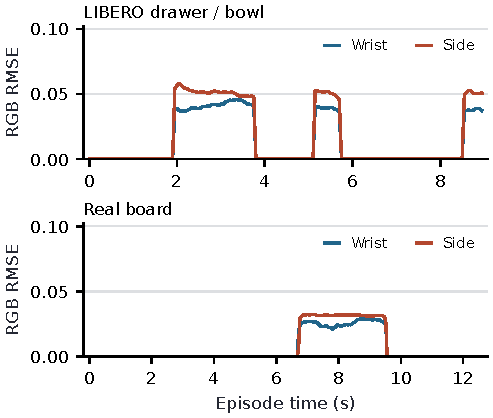
\includegraphics[width=\columnwidth]{decoder_modulation.pdf}
  \caption{Decoder spatial modulation on versus off. Curves are framewise
  RGB RMSE between paired renders for the wrist and side cameras. Inputs,
  weights, attention and gates are fixed. Episode 0 contains 180 simulated
  anchors and 316 real-board anchors. Flat intervals indicate identical
  pixels under this bypass.}
  \label{fig:decoder_modulation}
\end{figure}

\subsection{Closed-loop test of a simulation-trained teacher}
In a separate LIBERO Kitchen Scene 4 run, the task is to close the bottom
drawer and open the top drawer. The teacher has two residual CA blocks
and a 20-sample causal wrench history. With 10\% of episodes reserved
for validation, raw action MSE fell from 0.04716 at step 3,220 to
0.02419 at step 200,000 (Fig.~\ref{fig:k4_validation}). The archived
200k evaluation records \textbf{0 successes in 50 rollouts} with IK
joint control, incremental gripper commands and a limit of 400 control
frames per rollout. This evaluation tests one teacher and controller.
It provides no paired RGB/CIVI comparison for the simulated task.
Table~\ref{tab:success} reports the real-robot paired policy comparisons.

\begin{figure}[t]
  \centering
  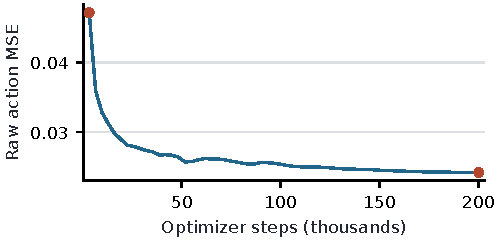
\includegraphics[width=\columnwidth]{libero_k4_validation.pdf}
  \caption{Held-out action prediction during K4 teacher training. Each
  point is a logged validation evaluation. The endpoint is the 200k-step
  checkpoint in the rollout study.}
  \label{fig:k4_validation}
\end{figure}

\section{Repository Index}
\label{sec:index}
\begingroup\small\sloppy
The source figures are copied from \texttt{docs/figures/method} and
\texttt{docs/figures/analysis}. The quantitative records are under
\texttt{data/debug}, notably the experiment directories
\texttt{torque\_response\_eval\_01}, \texttt{phase\_gate\_ce\_search\_01},
\texttt{image\_tau\_phase\_gate\_02}, \texttt{student\_ffn\_quick\_01},
\texttt{full\_data\_paired\_distill\_02},
\texttt{student\_latent\_distillation},
\texttt{2026.11.15/student\_dual\_path\_ablation},
\texttt{tau\_ext\_momentum\_vs\_rnea\_20261118\_204703},
\texttt{tau\_capacity\_v2}, and \texttt{civi\_student\_iteration}. Each
experiment directory contains manifests, raw metrics, and relevant
configurations. The task-sequence figure is copied from
\texttt{docs/figures/method/assets}. The companion source index in the
supplement folder identifies the archived arrays, checkpoints, selected
observations and metric definitions for Sections~\ref{sec:fusion_probes}
and~\ref{sec:sim_real}.
\par\endgroup

\begin{thebibliography}{4}
\bibitem{black2025}
K. Black et al. $\pi_0$: A vision-language-action flow model for general robot
control. In \emph{RSS}, 2025.

\bibitem{chi2023}
C. Chi et al. Diffusion policy: Visuomotor policy learning via action diffusion.
In \emph{RSS}, 2023.

\bibitem{oh2026}
S. Oh et al. FACTR 2: Learning external force sensing for commodity robot arms
improves policy learning. 2026.

\bibitem{simeoni2025}
O. Simeoni et al. DINOv3. 2025.
\end{thebibliography}

\end{document}
